
% Default to the notebook output style

    


% Inherit from the specified cell style.




    
\documentclass[11pt]{article}

    
    
    \usepackage[T1]{fontenc}
    % Nicer default font (+ math font) than Computer Modern for most use cases
    \usepackage{mathpazo}

    % Basic figure setup, for now with no caption control since it's done
    % automatically by Pandoc (which extracts ![](path) syntax from Markdown).
    \usepackage{graphicx}
    % We will generate all images so they have a width \maxwidth. This means
    % that they will get their normal width if they fit onto the page, but
    % are scaled down if they would overflow the margins.
    \makeatletter
    \def\maxwidth{\ifdim\Gin@nat@width>\linewidth\linewidth
    \else\Gin@nat@width\fi}
    \makeatother
    \let\Oldincludegraphics\includegraphics
    % Set max figure width to be 80% of text width, for now hardcoded.
    \renewcommand{\includegraphics}[1]{\Oldincludegraphics[width=.8\maxwidth]{#1}}
    % Ensure that by default, figures have no caption (until we provide a
    % proper Figure object with a Caption API and a way to capture that
    % in the conversion process - todo).
    \usepackage{caption}
    \DeclareCaptionLabelFormat{nolabel}{}
    \captionsetup{labelformat=nolabel}

    \usepackage{adjustbox} % Used to constrain images to a maximum size 
    \usepackage{xcolor} % Allow colors to be defined
    \usepackage{enumerate} % Needed for markdown enumerations to work
    \usepackage{geometry} % Used to adjust the document margins
    \usepackage{amsmath} % Equations
    \usepackage{amssymb} % Equations
    \usepackage{textcomp} % defines textquotesingle
    % Hack from http://tex.stackexchange.com/a/47451/13684:
    \AtBeginDocument{%
        \def\PYZsq{\textquotesingle}% Upright quotes in Pygmentized code
    }
    \usepackage{upquote} % Upright quotes for verbatim code
    \usepackage{eurosym} % defines \euro
    \usepackage[mathletters]{ucs} % Extended unicode (utf-8) support
    \usepackage[utf8x]{inputenc} % Allow utf-8 characters in the tex document
    \usepackage{fancyvrb} % verbatim replacement that allows latex
    \usepackage{grffile} % extends the file name processing of package graphics 
                         % to support a larger range 
    % The hyperref package gives us a pdf with properly built
    % internal navigation ('pdf bookmarks' for the table of contents,
    % internal cross-reference links, web links for URLs, etc.)
    \usepackage{hyperref}
    \usepackage{longtable} % longtable support required by pandoc >1.10
    \usepackage{booktabs}  % table support for pandoc > 1.12.2
    \usepackage[inline]{enumitem} % IRkernel/repr support (it uses the enumerate* environment)
    \usepackage[normalem]{ulem} % ulem is needed to support strikethroughs (\sout)
                                % normalem makes italics be italics, not underlines
    

    
    
    % Colors for the hyperref package
    \definecolor{urlcolor}{rgb}{0,.145,.698}
    \definecolor{linkcolor}{rgb}{.71,0.21,0.01}
    \definecolor{citecolor}{rgb}{.12,.54,.11}

    % ANSI colors
    \definecolor{ansi-black}{HTML}{3E424D}
    \definecolor{ansi-black-intense}{HTML}{282C36}
    \definecolor{ansi-red}{HTML}{E75C58}
    \definecolor{ansi-red-intense}{HTML}{B22B31}
    \definecolor{ansi-green}{HTML}{00A250}
    \definecolor{ansi-green-intense}{HTML}{007427}
    \definecolor{ansi-yellow}{HTML}{DDB62B}
    \definecolor{ansi-yellow-intense}{HTML}{B27D12}
    \definecolor{ansi-blue}{HTML}{208FFB}
    \definecolor{ansi-blue-intense}{HTML}{0065CA}
    \definecolor{ansi-magenta}{HTML}{D160C4}
    \definecolor{ansi-magenta-intense}{HTML}{A03196}
    \definecolor{ansi-cyan}{HTML}{60C6C8}
    \definecolor{ansi-cyan-intense}{HTML}{258F8F}
    \definecolor{ansi-white}{HTML}{C5C1B4}
    \definecolor{ansi-white-intense}{HTML}{A1A6B2}

    % commands and environments needed by pandoc snippets
    % extracted from the output of `pandoc -s`
    \providecommand{\tightlist}{%
      \setlength{\itemsep}{0pt}\setlength{\parskip}{0pt}}
    \DefineVerbatimEnvironment{Highlighting}{Verbatim}{commandchars=\\\{\}}
    % Add ',fontsize=\small' for more characters per line
    \newenvironment{Shaded}{}{}
    \newcommand{\KeywordTok}[1]{\textcolor[rgb]{0.00,0.44,0.13}{\textbf{{#1}}}}
    \newcommand{\DataTypeTok}[1]{\textcolor[rgb]{0.56,0.13,0.00}{{#1}}}
    \newcommand{\DecValTok}[1]{\textcolor[rgb]{0.25,0.63,0.44}{{#1}}}
    \newcommand{\BaseNTok}[1]{\textcolor[rgb]{0.25,0.63,0.44}{{#1}}}
    \newcommand{\FloatTok}[1]{\textcolor[rgb]{0.25,0.63,0.44}{{#1}}}
    \newcommand{\CharTok}[1]{\textcolor[rgb]{0.25,0.44,0.63}{{#1}}}
    \newcommand{\StringTok}[1]{\textcolor[rgb]{0.25,0.44,0.63}{{#1}}}
    \newcommand{\CommentTok}[1]{\textcolor[rgb]{0.38,0.63,0.69}{\textit{{#1}}}}
    \newcommand{\OtherTok}[1]{\textcolor[rgb]{0.00,0.44,0.13}{{#1}}}
    \newcommand{\AlertTok}[1]{\textcolor[rgb]{1.00,0.00,0.00}{\textbf{{#1}}}}
    \newcommand{\FunctionTok}[1]{\textcolor[rgb]{0.02,0.16,0.49}{{#1}}}
    \newcommand{\RegionMarkerTok}[1]{{#1}}
    \newcommand{\ErrorTok}[1]{\textcolor[rgb]{1.00,0.00,0.00}{\textbf{{#1}}}}
    \newcommand{\NormalTok}[1]{{#1}}
    
    % Additional commands for more recent versions of Pandoc
    \newcommand{\ConstantTok}[1]{\textcolor[rgb]{0.53,0.00,0.00}{{#1}}}
    \newcommand{\SpecialCharTok}[1]{\textcolor[rgb]{0.25,0.44,0.63}{{#1}}}
    \newcommand{\VerbatimStringTok}[1]{\textcolor[rgb]{0.25,0.44,0.63}{{#1}}}
    \newcommand{\SpecialStringTok}[1]{\textcolor[rgb]{0.73,0.40,0.53}{{#1}}}
    \newcommand{\ImportTok}[1]{{#1}}
    \newcommand{\DocumentationTok}[1]{\textcolor[rgb]{0.73,0.13,0.13}{\textit{{#1}}}}
    \newcommand{\AnnotationTok}[1]{\textcolor[rgb]{0.38,0.63,0.69}{\textbf{\textit{{#1}}}}}
    \newcommand{\CommentVarTok}[1]{\textcolor[rgb]{0.38,0.63,0.69}{\textbf{\textit{{#1}}}}}
    \newcommand{\VariableTok}[1]{\textcolor[rgb]{0.10,0.09,0.49}{{#1}}}
    \newcommand{\ControlFlowTok}[1]{\textcolor[rgb]{0.00,0.44,0.13}{\textbf{{#1}}}}
    \newcommand{\OperatorTok}[1]{\textcolor[rgb]{0.40,0.40,0.40}{{#1}}}
    \newcommand{\BuiltInTok}[1]{{#1}}
    \newcommand{\ExtensionTok}[1]{{#1}}
    \newcommand{\PreprocessorTok}[1]{\textcolor[rgb]{0.74,0.48,0.00}{{#1}}}
    \newcommand{\AttributeTok}[1]{\textcolor[rgb]{0.49,0.56,0.16}{{#1}}}
    \newcommand{\InformationTok}[1]{\textcolor[rgb]{0.38,0.63,0.69}{\textbf{\textit{{#1}}}}}
    \newcommand{\WarningTok}[1]{\textcolor[rgb]{0.38,0.63,0.69}{\textbf{\textit{{#1}}}}}
    
    
    % Define a nice break command that doesn't care if a line doesn't already
    % exist.
    \def\br{\hspace*{\fill} \\* }
    % Math Jax compatability definitions
    \def\gt{>}
    \def\lt{<}
    % Document parameters
    \title{Lab2\_DL-Students}
    
    
    

    % Pygments definitions
    
\makeatletter
\def\PY@reset{\let\PY@it=\relax \let\PY@bf=\relax%
    \let\PY@ul=\relax \let\PY@tc=\relax%
    \let\PY@bc=\relax \let\PY@ff=\relax}
\def\PY@tok#1{\csname PY@tok@#1\endcsname}
\def\PY@toks#1+{\ifx\relax#1\empty\else%
    \PY@tok{#1}\expandafter\PY@toks\fi}
\def\PY@do#1{\PY@bc{\PY@tc{\PY@ul{%
    \PY@it{\PY@bf{\PY@ff{#1}}}}}}}
\def\PY#1#2{\PY@reset\PY@toks#1+\relax+\PY@do{#2}}

\expandafter\def\csname PY@tok@gh\endcsname{\let\PY@bf=\textbf\def\PY@tc##1{\textcolor[rgb]{0.00,0.00,0.50}{##1}}}
\expandafter\def\csname PY@tok@sb\endcsname{\def\PY@tc##1{\textcolor[rgb]{0.73,0.13,0.13}{##1}}}
\expandafter\def\csname PY@tok@cpf\endcsname{\let\PY@it=\textit\def\PY@tc##1{\textcolor[rgb]{0.25,0.50,0.50}{##1}}}
\expandafter\def\csname PY@tok@gr\endcsname{\def\PY@tc##1{\textcolor[rgb]{1.00,0.00,0.00}{##1}}}
\expandafter\def\csname PY@tok@ow\endcsname{\let\PY@bf=\textbf\def\PY@tc##1{\textcolor[rgb]{0.67,0.13,1.00}{##1}}}
\expandafter\def\csname PY@tok@fm\endcsname{\def\PY@tc##1{\textcolor[rgb]{0.00,0.00,1.00}{##1}}}
\expandafter\def\csname PY@tok@kr\endcsname{\let\PY@bf=\textbf\def\PY@tc##1{\textcolor[rgb]{0.00,0.50,0.00}{##1}}}
\expandafter\def\csname PY@tok@nn\endcsname{\let\PY@bf=\textbf\def\PY@tc##1{\textcolor[rgb]{0.00,0.00,1.00}{##1}}}
\expandafter\def\csname PY@tok@nl\endcsname{\def\PY@tc##1{\textcolor[rgb]{0.63,0.63,0.00}{##1}}}
\expandafter\def\csname PY@tok@ge\endcsname{\let\PY@it=\textit}
\expandafter\def\csname PY@tok@vm\endcsname{\def\PY@tc##1{\textcolor[rgb]{0.10,0.09,0.49}{##1}}}
\expandafter\def\csname PY@tok@nb\endcsname{\def\PY@tc##1{\textcolor[rgb]{0.00,0.50,0.00}{##1}}}
\expandafter\def\csname PY@tok@kt\endcsname{\def\PY@tc##1{\textcolor[rgb]{0.69,0.00,0.25}{##1}}}
\expandafter\def\csname PY@tok@sd\endcsname{\let\PY@it=\textit\def\PY@tc##1{\textcolor[rgb]{0.73,0.13,0.13}{##1}}}
\expandafter\def\csname PY@tok@se\endcsname{\let\PY@bf=\textbf\def\PY@tc##1{\textcolor[rgb]{0.73,0.40,0.13}{##1}}}
\expandafter\def\csname PY@tok@bp\endcsname{\def\PY@tc##1{\textcolor[rgb]{0.00,0.50,0.00}{##1}}}
\expandafter\def\csname PY@tok@gi\endcsname{\def\PY@tc##1{\textcolor[rgb]{0.00,0.63,0.00}{##1}}}
\expandafter\def\csname PY@tok@mb\endcsname{\def\PY@tc##1{\textcolor[rgb]{0.40,0.40,0.40}{##1}}}
\expandafter\def\csname PY@tok@nf\endcsname{\def\PY@tc##1{\textcolor[rgb]{0.00,0.00,1.00}{##1}}}
\expandafter\def\csname PY@tok@mi\endcsname{\def\PY@tc##1{\textcolor[rgb]{0.40,0.40,0.40}{##1}}}
\expandafter\def\csname PY@tok@c\endcsname{\let\PY@it=\textit\def\PY@tc##1{\textcolor[rgb]{0.25,0.50,0.50}{##1}}}
\expandafter\def\csname PY@tok@o\endcsname{\def\PY@tc##1{\textcolor[rgb]{0.40,0.40,0.40}{##1}}}
\expandafter\def\csname PY@tok@mh\endcsname{\def\PY@tc##1{\textcolor[rgb]{0.40,0.40,0.40}{##1}}}
\expandafter\def\csname PY@tok@gp\endcsname{\let\PY@bf=\textbf\def\PY@tc##1{\textcolor[rgb]{0.00,0.00,0.50}{##1}}}
\expandafter\def\csname PY@tok@s\endcsname{\def\PY@tc##1{\textcolor[rgb]{0.73,0.13,0.13}{##1}}}
\expandafter\def\csname PY@tok@kc\endcsname{\let\PY@bf=\textbf\def\PY@tc##1{\textcolor[rgb]{0.00,0.50,0.00}{##1}}}
\expandafter\def\csname PY@tok@cm\endcsname{\let\PY@it=\textit\def\PY@tc##1{\textcolor[rgb]{0.25,0.50,0.50}{##1}}}
\expandafter\def\csname PY@tok@kp\endcsname{\def\PY@tc##1{\textcolor[rgb]{0.00,0.50,0.00}{##1}}}
\expandafter\def\csname PY@tok@si\endcsname{\let\PY@bf=\textbf\def\PY@tc##1{\textcolor[rgb]{0.73,0.40,0.53}{##1}}}
\expandafter\def\csname PY@tok@m\endcsname{\def\PY@tc##1{\textcolor[rgb]{0.40,0.40,0.40}{##1}}}
\expandafter\def\csname PY@tok@ne\endcsname{\let\PY@bf=\textbf\def\PY@tc##1{\textcolor[rgb]{0.82,0.25,0.23}{##1}}}
\expandafter\def\csname PY@tok@gs\endcsname{\let\PY@bf=\textbf}
\expandafter\def\csname PY@tok@err\endcsname{\def\PY@bc##1{\setlength{\fboxsep}{0pt}\fcolorbox[rgb]{1.00,0.00,0.00}{1,1,1}{\strut ##1}}}
\expandafter\def\csname PY@tok@go\endcsname{\def\PY@tc##1{\textcolor[rgb]{0.53,0.53,0.53}{##1}}}
\expandafter\def\csname PY@tok@sa\endcsname{\def\PY@tc##1{\textcolor[rgb]{0.73,0.13,0.13}{##1}}}
\expandafter\def\csname PY@tok@nc\endcsname{\let\PY@bf=\textbf\def\PY@tc##1{\textcolor[rgb]{0.00,0.00,1.00}{##1}}}
\expandafter\def\csname PY@tok@k\endcsname{\let\PY@bf=\textbf\def\PY@tc##1{\textcolor[rgb]{0.00,0.50,0.00}{##1}}}
\expandafter\def\csname PY@tok@dl\endcsname{\def\PY@tc##1{\textcolor[rgb]{0.73,0.13,0.13}{##1}}}
\expandafter\def\csname PY@tok@ni\endcsname{\let\PY@bf=\textbf\def\PY@tc##1{\textcolor[rgb]{0.60,0.60,0.60}{##1}}}
\expandafter\def\csname PY@tok@w\endcsname{\def\PY@tc##1{\textcolor[rgb]{0.73,0.73,0.73}{##1}}}
\expandafter\def\csname PY@tok@mo\endcsname{\def\PY@tc##1{\textcolor[rgb]{0.40,0.40,0.40}{##1}}}
\expandafter\def\csname PY@tok@vc\endcsname{\def\PY@tc##1{\textcolor[rgb]{0.10,0.09,0.49}{##1}}}
\expandafter\def\csname PY@tok@mf\endcsname{\def\PY@tc##1{\textcolor[rgb]{0.40,0.40,0.40}{##1}}}
\expandafter\def\csname PY@tok@sr\endcsname{\def\PY@tc##1{\textcolor[rgb]{0.73,0.40,0.53}{##1}}}
\expandafter\def\csname PY@tok@ss\endcsname{\def\PY@tc##1{\textcolor[rgb]{0.10,0.09,0.49}{##1}}}
\expandafter\def\csname PY@tok@vg\endcsname{\def\PY@tc##1{\textcolor[rgb]{0.10,0.09,0.49}{##1}}}
\expandafter\def\csname PY@tok@c1\endcsname{\let\PY@it=\textit\def\PY@tc##1{\textcolor[rgb]{0.25,0.50,0.50}{##1}}}
\expandafter\def\csname PY@tok@nd\endcsname{\def\PY@tc##1{\textcolor[rgb]{0.67,0.13,1.00}{##1}}}
\expandafter\def\csname PY@tok@no\endcsname{\def\PY@tc##1{\textcolor[rgb]{0.53,0.00,0.00}{##1}}}
\expandafter\def\csname PY@tok@vi\endcsname{\def\PY@tc##1{\textcolor[rgb]{0.10,0.09,0.49}{##1}}}
\expandafter\def\csname PY@tok@cp\endcsname{\def\PY@tc##1{\textcolor[rgb]{0.74,0.48,0.00}{##1}}}
\expandafter\def\csname PY@tok@sc\endcsname{\def\PY@tc##1{\textcolor[rgb]{0.73,0.13,0.13}{##1}}}
\expandafter\def\csname PY@tok@gt\endcsname{\def\PY@tc##1{\textcolor[rgb]{0.00,0.27,0.87}{##1}}}
\expandafter\def\csname PY@tok@na\endcsname{\def\PY@tc##1{\textcolor[rgb]{0.49,0.56,0.16}{##1}}}
\expandafter\def\csname PY@tok@s1\endcsname{\def\PY@tc##1{\textcolor[rgb]{0.73,0.13,0.13}{##1}}}
\expandafter\def\csname PY@tok@sx\endcsname{\def\PY@tc##1{\textcolor[rgb]{0.00,0.50,0.00}{##1}}}
\expandafter\def\csname PY@tok@nv\endcsname{\def\PY@tc##1{\textcolor[rgb]{0.10,0.09,0.49}{##1}}}
\expandafter\def\csname PY@tok@gd\endcsname{\def\PY@tc##1{\textcolor[rgb]{0.63,0.00,0.00}{##1}}}
\expandafter\def\csname PY@tok@kd\endcsname{\let\PY@bf=\textbf\def\PY@tc##1{\textcolor[rgb]{0.00,0.50,0.00}{##1}}}
\expandafter\def\csname PY@tok@ch\endcsname{\let\PY@it=\textit\def\PY@tc##1{\textcolor[rgb]{0.25,0.50,0.50}{##1}}}
\expandafter\def\csname PY@tok@cs\endcsname{\let\PY@it=\textit\def\PY@tc##1{\textcolor[rgb]{0.25,0.50,0.50}{##1}}}
\expandafter\def\csname PY@tok@gu\endcsname{\let\PY@bf=\textbf\def\PY@tc##1{\textcolor[rgb]{0.50,0.00,0.50}{##1}}}
\expandafter\def\csname PY@tok@kn\endcsname{\let\PY@bf=\textbf\def\PY@tc##1{\textcolor[rgb]{0.00,0.50,0.00}{##1}}}
\expandafter\def\csname PY@tok@il\endcsname{\def\PY@tc##1{\textcolor[rgb]{0.40,0.40,0.40}{##1}}}
\expandafter\def\csname PY@tok@sh\endcsname{\def\PY@tc##1{\textcolor[rgb]{0.73,0.13,0.13}{##1}}}
\expandafter\def\csname PY@tok@s2\endcsname{\def\PY@tc##1{\textcolor[rgb]{0.73,0.13,0.13}{##1}}}
\expandafter\def\csname PY@tok@nt\endcsname{\let\PY@bf=\textbf\def\PY@tc##1{\textcolor[rgb]{0.00,0.50,0.00}{##1}}}

\def\PYZbs{\char`\\}
\def\PYZus{\char`\_}
\def\PYZob{\char`\{}
\def\PYZcb{\char`\}}
\def\PYZca{\char`\^}
\def\PYZam{\char`\&}
\def\PYZlt{\char`\<}
\def\PYZgt{\char`\>}
\def\PYZsh{\char`\#}
\def\PYZpc{\char`\%}
\def\PYZdl{\char`\$}
\def\PYZhy{\char`\-}
\def\PYZsq{\char`\'}
\def\PYZdq{\char`\"}
\def\PYZti{\char`\~}
% for compatibility with earlier versions
\def\PYZat{@}
\def\PYZlb{[}
\def\PYZrb{]}
\makeatother


    % Exact colors from NB
    \definecolor{incolor}{rgb}{0.0, 0.0, 0.5}
    \definecolor{outcolor}{rgb}{0.545, 0.0, 0.0}



    
    % Prevent overflowing lines due to hard-to-break entities
    \sloppy 
    % Setup hyperref package
    \hypersetup{
      breaklinks=true,  % so long urls are correctly broken across lines
      colorlinks=true,
      urlcolor=urlcolor,
      linkcolor=linkcolor,
      citecolor=citecolor,
      }
    % Slightly bigger margins than the latex defaults
    
    \geometry{verbose,tmargin=1in,bmargin=1in,lmargin=1in,rmargin=1in}
    
    

    \begin{document}
    
    
    \maketitle
    
    

    
    Deep Learning

Lab Session 2 - 1.5 Hours

Convolutional Neural Network (CNN) for Handwritten Digits Recognition

     Group name: deeplearn25

The aim of this session is to practice with Convolutional Neural
Networks. Each group should fill and run appropriate notebook cells.

Generate your final report (export as HTML) and upload it on the
submission website http://bigfoot-m1.eurecom.fr/teachingsub/login (using
your deeplearnXX/password). Do not forget to run all your cells before
generating your final report and do not forget to include the names of
all participants in the group. The lab session should be completed and
submitted by May 30th 2018 (23:59:59 CET).

    \section{Introduction}\label{introduction}

    In the previous Lab Session, you built a Multilayer Perceptron for
recognizing hand-written digits from the MNIST data-set. The best
achieved accuracy on testing data was about 97\%. Can you do better than
these results using a deep CNN ? In this Lab Session, you will build,
train and optimize in TensorFlow one of the early Convolutional Neural
Networks, \textbf{LeNet-5}, to go to more than 99\% of accuracy.

    \begin{Verbatim}[commandchars=\\\{\}]
{\color{incolor}In [{\color{incolor}1}]:} \PY{k+kn}{import} \PY{n+nn}{warnings}
        \PY{n}{warnings}\PY{o}{.}\PY{n}{simplefilter}\PY{p}{(}\PY{l+s+s2}{\PYZdq{}}\PY{l+s+s2}{ignore}\PY{l+s+s2}{\PYZdq{}}\PY{p}{)}
\end{Verbatim}


    \section{Load MNIST Data in
TensorFlow}\label{load-mnist-data-in-tensorflow}

Run the cell below to load the MNIST data that comes with TensorFlow.
You will use this data in \textbf{Section 1} and \textbf{Section 2}.

    \begin{Verbatim}[commandchars=\\\{\}]
{\color{incolor}In [{\color{incolor}2}]:} \PY{k+kn}{import} \PY{n+nn}{tensorflow} \PY{k}{as} \PY{n+nn}{tf}
        \PY{k+kn}{import} \PY{n+nn}{numpy} \PY{k}{as} \PY{n+nn}{np}
        \PY{k+kn}{from} \PY{n+nn}{tensorflow}\PY{n+nn}{.}\PY{n+nn}{examples}\PY{n+nn}{.}\PY{n+nn}{tutorials}\PY{n+nn}{.}\PY{n+nn}{mnist} \PY{k}{import} \PY{n}{input\PYZus{}data}
        \PY{n}{mnist} \PY{o}{=} \PY{n}{input\PYZus{}data}\PY{o}{.}\PY{n}{read\PYZus{}data\PYZus{}sets}\PY{p}{(}\PY{l+s+s2}{\PYZdq{}}\PY{l+s+s2}{MNIST\PYZus{}data/}\PY{l+s+s2}{\PYZdq{}}\PY{p}{,} \PY{n}{one\PYZus{}hot}\PY{o}{=}\PY{k+kc}{True}\PY{p}{)}
        \PY{n}{X\PYZus{}train}\PY{p}{,} \PY{n}{y\PYZus{}train}           \PY{o}{=} \PY{n}{mnist}\PY{o}{.}\PY{n}{train}\PY{o}{.}\PY{n}{images}\PY{p}{,} \PY{n}{mnist}\PY{o}{.}\PY{n}{train}\PY{o}{.}\PY{n}{labels}
        \PY{n}{X\PYZus{}validation}\PY{p}{,} \PY{n}{y\PYZus{}validation} \PY{o}{=} \PY{n}{mnist}\PY{o}{.}\PY{n}{validation}\PY{o}{.}\PY{n}{images}\PY{p}{,} \PY{n}{mnist}\PY{o}{.}\PY{n}{validation}\PY{o}{.}\PY{n}{labels}
        \PY{n}{X\PYZus{}test}\PY{p}{,} \PY{n}{y\PYZus{}test}             \PY{o}{=} \PY{n}{mnist}\PY{o}{.}\PY{n}{test}\PY{o}{.}\PY{n}{images}\PY{p}{,} \PY{n}{mnist}\PY{o}{.}\PY{n}{test}\PY{o}{.}\PY{n}{labels}
        \PY{n+nb}{print}\PY{p}{(}\PY{l+s+s2}{\PYZdq{}}\PY{l+s+s2}{Image Shape: }\PY{l+s+si}{\PYZob{}\PYZcb{}}\PY{l+s+s2}{\PYZdq{}}\PY{o}{.}\PY{n}{format}\PY{p}{(}\PY{n}{X\PYZus{}train}\PY{p}{[}\PY{l+m+mi}{0}\PY{p}{]}\PY{o}{.}\PY{n}{shape}\PY{p}{)}\PY{p}{)}
        \PY{n+nb}{print}\PY{p}{(}\PY{l+s+s2}{\PYZdq{}}\PY{l+s+s2}{Training Set:   }\PY{l+s+si}{\PYZob{}\PYZcb{}}\PY{l+s+s2}{ samples}\PY{l+s+s2}{\PYZdq{}}\PY{o}{.}\PY{n}{format}\PY{p}{(}\PY{n+nb}{len}\PY{p}{(}\PY{n}{X\PYZus{}train}\PY{p}{)}\PY{p}{)}\PY{p}{)}
        \PY{n+nb}{print}\PY{p}{(}\PY{l+s+s2}{\PYZdq{}}\PY{l+s+s2}{Validation Set: }\PY{l+s+si}{\PYZob{}\PYZcb{}}\PY{l+s+s2}{ samples}\PY{l+s+s2}{\PYZdq{}}\PY{o}{.}\PY{n}{format}\PY{p}{(}\PY{n+nb}{len}\PY{p}{(}\PY{n}{X\PYZus{}validation}\PY{p}{)}\PY{p}{)}\PY{p}{)}
        \PY{n+nb}{print}\PY{p}{(}\PY{l+s+s2}{\PYZdq{}}\PY{l+s+s2}{Test Set:       }\PY{l+s+si}{\PYZob{}\PYZcb{}}\PY{l+s+s2}{ samples}\PY{l+s+s2}{\PYZdq{}}\PY{o}{.}\PY{n}{format}\PY{p}{(}\PY{n+nb}{len}\PY{p}{(}\PY{n}{X\PYZus{}test}\PY{p}{)}\PY{p}{)}\PY{p}{)}
        
        \PY{n}{epsilon} \PY{o}{=} \PY{l+m+mf}{1e\PYZhy{}10} \PY{c+c1}{\PYZsh{} this is a parameter you will use later}
\end{Verbatim}


    \begin{Verbatim}[commandchars=\\\{\}]
Extracting MNIST\_data/train-images-idx3-ubyte.gz
Extracting MNIST\_data/train-labels-idx1-ubyte.gz
Extracting MNIST\_data/t10k-images-idx3-ubyte.gz
Extracting MNIST\_data/t10k-labels-idx1-ubyte.gz
Image Shape: (784,)
Training Set:   55000 samples
Validation Set: 5000 samples
Test Set:       10000 samples

    \end{Verbatim}

    \section{Section 1 : My First Model in
TensorFlow}\label{section-1-my-first-model-in-tensorflow}

    Before starting with CNN, let's train and test in TensorFlow the example
\textbf{y=softmax(Wx+b)} seen in the first lab.

This model reaches an accuracy of about 92 \%. You will also learn how
to launch the TensorBoard
https://www.tensorflow.org/get\_started/summaries\_and\_tensorboard to
visualize the computation graph, statistics and learning curves.

     Part 1 : Read carefully the code in the cell below. Run it to perform
training.

    \begin{Verbatim}[commandchars=\\\{\}]
{\color{incolor}In [{\color{incolor}3}]:} \PY{c+c1}{\PYZsh{}STEP 1}
        
        \PY{c+c1}{\PYZsh{} Parameters}
        \PY{n}{learning\PYZus{}rate} \PY{o}{=} \PY{l+m+mf}{0.01}
        \PY{n}{training\PYZus{}epochs} \PY{o}{=} \PY{l+m+mi}{40}
        \PY{n}{batch\PYZus{}size} \PY{o}{=} \PY{l+m+mi}{128}
        \PY{n}{display\PYZus{}step} \PY{o}{=} \PY{l+m+mi}{10}
        \PY{n}{logs\PYZus{}path} \PY{o}{=} \PY{l+s+s1}{\PYZsq{}}\PY{l+s+s1}{log\PYZus{}files/}\PY{l+s+s1}{\PYZsq{}}  \PY{c+c1}{\PYZsh{} useful for tensorboard}
        
        \PY{c+c1}{\PYZsh{} tf Graph Input:  mnist data image of shape 28*28=784}
        \PY{n}{x} \PY{o}{=} \PY{n}{tf}\PY{o}{.}\PY{n}{placeholder}\PY{p}{(}\PY{n}{tf}\PY{o}{.}\PY{n}{float32}\PY{p}{,} \PY{p}{[}\PY{k+kc}{None}\PY{p}{,} \PY{l+m+mi}{784}\PY{p}{]}\PY{p}{,} \PY{n}{name}\PY{o}{=}\PY{l+s+s1}{\PYZsq{}}\PY{l+s+s1}{InputData}\PY{l+s+s1}{\PYZsq{}}\PY{p}{)}
        \PY{c+c1}{\PYZsh{} 0\PYZhy{}9 digits recognition,  10 classes}
        \PY{n}{y} \PY{o}{=} \PY{n}{tf}\PY{o}{.}\PY{n}{placeholder}\PY{p}{(}\PY{n}{tf}\PY{o}{.}\PY{n}{float32}\PY{p}{,} \PY{p}{[}\PY{k+kc}{None}\PY{p}{,} \PY{l+m+mi}{10}\PY{p}{]}\PY{p}{,} \PY{n}{name}\PY{o}{=}\PY{l+s+s1}{\PYZsq{}}\PY{l+s+s1}{LabelData}\PY{l+s+s1}{\PYZsq{}}\PY{p}{)}
        
        \PY{c+c1}{\PYZsh{} Set model weights}
        \PY{n}{W} \PY{o}{=} \PY{n}{tf}\PY{o}{.}\PY{n}{Variable}\PY{p}{(}\PY{n}{tf}\PY{o}{.}\PY{n}{zeros}\PY{p}{(}\PY{p}{[}\PY{l+m+mi}{784}\PY{p}{,} \PY{l+m+mi}{10}\PY{p}{]}\PY{p}{)}\PY{p}{,} \PY{n}{name}\PY{o}{=}\PY{l+s+s1}{\PYZsq{}}\PY{l+s+s1}{Weights}\PY{l+s+s1}{\PYZsq{}}\PY{p}{)}
        \PY{n}{b} \PY{o}{=} \PY{n}{tf}\PY{o}{.}\PY{n}{Variable}\PY{p}{(}\PY{n}{tf}\PY{o}{.}\PY{n}{zeros}\PY{p}{(}\PY{p}{[}\PY{l+m+mi}{10}\PY{p}{]}\PY{p}{)}\PY{p}{,} \PY{n}{name}\PY{o}{=}\PY{l+s+s1}{\PYZsq{}}\PY{l+s+s1}{Bias}\PY{l+s+s1}{\PYZsq{}}\PY{p}{)}
        
        \PY{c+c1}{\PYZsh{} Construct model and encapsulating all ops into scopes, making Tensorboard\PYZsq{}s Graph visualization more convenient}
        \PY{k}{with} \PY{n}{tf}\PY{o}{.}\PY{n}{name\PYZus{}scope}\PY{p}{(}\PY{l+s+s1}{\PYZsq{}}\PY{l+s+s1}{Model}\PY{l+s+s1}{\PYZsq{}}\PY{p}{)}\PY{p}{:}
            \PY{c+c1}{\PYZsh{} Model}
            \PY{n}{pred} \PY{o}{=} \PY{n}{tf}\PY{o}{.}\PY{n}{nn}\PY{o}{.}\PY{n}{softmax}\PY{p}{(}\PY{n}{tf}\PY{o}{.}\PY{n}{matmul}\PY{p}{(}\PY{n}{x}\PY{p}{,} \PY{n}{W}\PY{p}{)} \PY{o}{+} \PY{n}{b}\PY{p}{)} \PY{c+c1}{\PYZsh{} Softmax}
        \PY{k}{with} \PY{n}{tf}\PY{o}{.}\PY{n}{name\PYZus{}scope}\PY{p}{(}\PY{l+s+s1}{\PYZsq{}}\PY{l+s+s1}{Loss}\PY{l+s+s1}{\PYZsq{}}\PY{p}{)}\PY{p}{:}
            \PY{c+c1}{\PYZsh{} Minimize error using cross entropy}
            \PY{c+c1}{\PYZsh{} We use tf.clip\PYZus{}by\PYZus{}value to avoid having too low numbers in the log function}
            \PY{n}{cost} \PY{o}{=} \PY{n}{tf}\PY{o}{.}\PY{n}{reduce\PYZus{}mean}\PY{p}{(}\PY{o}{\PYZhy{}}\PY{n}{tf}\PY{o}{.}\PY{n}{reduce\PYZus{}sum}\PY{p}{(}\PY{n}{y}\PY{o}{*}\PY{n}{tf}\PY{o}{.}\PY{n}{log}\PY{p}{(}\PY{n}{tf}\PY{o}{.}\PY{n}{clip\PYZus{}by\PYZus{}value}\PY{p}{(}\PY{n}{pred}\PY{p}{,} \PY{n}{epsilon}\PY{p}{,} \PY{l+m+mf}{1.0}\PY{p}{)}\PY{p}{)}\PY{p}{,} \PY{n}{reduction\PYZus{}indices}\PY{o}{=}\PY{l+m+mi}{1}\PY{p}{)}\PY{p}{)}
        \PY{k}{with} \PY{n}{tf}\PY{o}{.}\PY{n}{name\PYZus{}scope}\PY{p}{(}\PY{l+s+s1}{\PYZsq{}}\PY{l+s+s1}{SGD}\PY{l+s+s1}{\PYZsq{}}\PY{p}{)}\PY{p}{:}
            \PY{c+c1}{\PYZsh{} Gradient Descent}
            \PY{n}{optimizer} \PY{o}{=} \PY{n}{tf}\PY{o}{.}\PY{n}{train}\PY{o}{.}\PY{n}{GradientDescentOptimizer}\PY{p}{(}\PY{n}{learning\PYZus{}rate}\PY{p}{)}\PY{o}{.}\PY{n}{minimize}\PY{p}{(}\PY{n}{cost}\PY{p}{)}
        \PY{k}{with} \PY{n}{tf}\PY{o}{.}\PY{n}{name\PYZus{}scope}\PY{p}{(}\PY{l+s+s1}{\PYZsq{}}\PY{l+s+s1}{Accuracy}\PY{l+s+s1}{\PYZsq{}}\PY{p}{)}\PY{p}{:}
            \PY{c+c1}{\PYZsh{} Accuracy}
            \PY{n}{acc} \PY{o}{=} \PY{n}{tf}\PY{o}{.}\PY{n}{equal}\PY{p}{(}\PY{n}{tf}\PY{o}{.}\PY{n}{argmax}\PY{p}{(}\PY{n}{pred}\PY{p}{,} \PY{l+m+mi}{1}\PY{p}{)}\PY{p}{,} \PY{n}{tf}\PY{o}{.}\PY{n}{argmax}\PY{p}{(}\PY{n}{y}\PY{p}{,} \PY{l+m+mi}{1}\PY{p}{)}\PY{p}{)}
            \PY{n}{acc} \PY{o}{=} \PY{n}{tf}\PY{o}{.}\PY{n}{reduce\PYZus{}mean}\PY{p}{(}\PY{n}{tf}\PY{o}{.}\PY{n}{cast}\PY{p}{(}\PY{n}{acc}\PY{p}{,} \PY{n}{tf}\PY{o}{.}\PY{n}{float32}\PY{p}{)}\PY{p}{)}
        
        \PY{c+c1}{\PYZsh{} Initializing the variables}
        \PY{n}{init} \PY{o}{=} \PY{n}{tf}\PY{o}{.}\PY{n}{global\PYZus{}variables\PYZus{}initializer}\PY{p}{(}\PY{p}{)}
        \PY{c+c1}{\PYZsh{} Create a summary to monitor cost tensor}
        \PY{n}{tf}\PY{o}{.}\PY{n}{summary}\PY{o}{.}\PY{n}{scalar}\PY{p}{(}\PY{l+s+s2}{\PYZdq{}}\PY{l+s+s2}{Loss}\PY{l+s+s2}{\PYZdq{}}\PY{p}{,} \PY{n}{cost}\PY{p}{)}
        \PY{c+c1}{\PYZsh{} Create a summary to monitor accuracy tensor}
        \PY{n}{tf}\PY{o}{.}\PY{n}{summary}\PY{o}{.}\PY{n}{scalar}\PY{p}{(}\PY{l+s+s2}{\PYZdq{}}\PY{l+s+s2}{Accuracy}\PY{l+s+s2}{\PYZdq{}}\PY{p}{,} \PY{n}{acc}\PY{p}{)}
        \PY{c+c1}{\PYZsh{} Merge all summaries into a single op}
        \PY{n}{merged\PYZus{}summary\PYZus{}op} \PY{o}{=} \PY{n}{tf}\PY{o}{.}\PY{n}{summary}\PY{o}{.}\PY{n}{merge\PYZus{}all}\PY{p}{(}\PY{p}{)}
        
        \PY{c+c1}{\PYZsh{}STEP 2 }
        
        \PY{c+c1}{\PYZsh{} Launch the graph for training}
        \PY{k}{with} \PY{n}{tf}\PY{o}{.}\PY{n}{Session}\PY{p}{(}\PY{p}{)} \PY{k}{as} \PY{n}{sess}\PY{p}{:}
            \PY{n}{sess}\PY{o}{.}\PY{n}{run}\PY{p}{(}\PY{n}{init}\PY{p}{)}
            \PY{c+c1}{\PYZsh{} op to write logs to Tensorboard}
            \PY{n}{summary\PYZus{}writer} \PY{o}{=} \PY{n}{tf}\PY{o}{.}\PY{n}{summary}\PY{o}{.}\PY{n}{FileWriter}\PY{p}{(}\PY{n}{logs\PYZus{}path}\PY{p}{,} \PY{n}{graph}\PY{o}{=}\PY{n}{tf}\PY{o}{.}\PY{n}{get\PYZus{}default\PYZus{}graph}\PY{p}{(}\PY{p}{)}\PY{p}{)}
            \PY{c+c1}{\PYZsh{} Training cycle}
            \PY{k}{for} \PY{n}{epoch} \PY{o+ow}{in} \PY{n+nb}{range}\PY{p}{(}\PY{n}{training\PYZus{}epochs}\PY{p}{)}\PY{p}{:}
                \PY{n}{avg\PYZus{}cost} \PY{o}{=} \PY{l+m+mf}{0.}
                \PY{n}{total\PYZus{}batch} \PY{o}{=} \PY{n+nb}{int}\PY{p}{(}\PY{n}{mnist}\PY{o}{.}\PY{n}{train}\PY{o}{.}\PY{n}{num\PYZus{}examples}\PY{o}{/}\PY{n}{batch\PYZus{}size}\PY{p}{)}
                \PY{c+c1}{\PYZsh{} Loop over all batches}
                \PY{k}{for} \PY{n}{i} \PY{o+ow}{in} \PY{n+nb}{range}\PY{p}{(}\PY{n}{total\PYZus{}batch}\PY{p}{)}\PY{p}{:}
                    \PY{n}{batch\PYZus{}xs}\PY{p}{,} \PY{n}{batch\PYZus{}ys} \PY{o}{=} \PY{n}{mnist}\PY{o}{.}\PY{n}{train}\PY{o}{.}\PY{n}{next\PYZus{}batch}\PY{p}{(}\PY{n}{batch\PYZus{}size}\PY{p}{,} \PY{n}{shuffle}\PY{o}{=}\PY{p}{(}\PY{n}{i}\PY{o}{==}\PY{l+m+mi}{0}\PY{p}{)}\PY{p}{)}
                    \PY{c+c1}{\PYZsh{} Run optimization op (backprop), cost op (to get loss value)}
                    \PY{c+c1}{\PYZsh{} and summary nodes}
                    \PY{n}{\PYZus{}}\PY{p}{,} \PY{n}{c}\PY{p}{,} \PY{n}{summary} \PY{o}{=} \PY{n}{sess}\PY{o}{.}\PY{n}{run}\PY{p}{(}\PY{p}{[}\PY{n}{optimizer}\PY{p}{,} \PY{n}{cost}\PY{p}{,} \PY{n}{merged\PYZus{}summary\PYZus{}op}\PY{p}{]}\PY{p}{,}
                                             \PY{n}{feed\PYZus{}dict}\PY{o}{=}\PY{p}{\PYZob{}}\PY{n}{x}\PY{p}{:} \PY{n}{batch\PYZus{}xs}\PY{p}{,} \PY{n}{y}\PY{p}{:} \PY{n}{batch\PYZus{}ys}\PY{p}{\PYZcb{}}\PY{p}{)}
                    \PY{c+c1}{\PYZsh{} Write logs at every iteration}
                    \PY{n}{summary\PYZus{}writer}\PY{o}{.}\PY{n}{add\PYZus{}summary}\PY{p}{(}\PY{n}{summary}\PY{p}{,} \PY{n}{epoch} \PY{o}{*} \PY{n}{total\PYZus{}batch} \PY{o}{+} \PY{n}{i}\PY{p}{)}
                    \PY{c+c1}{\PYZsh{} Compute average loss}
                    \PY{n}{avg\PYZus{}cost} \PY{o}{+}\PY{o}{=} \PY{n}{c} \PY{o}{/} \PY{n}{total\PYZus{}batch}
                \PY{c+c1}{\PYZsh{} Display logs per epoch step}
                \PY{k}{if} \PY{p}{(}\PY{n}{epoch}\PY{o}{+}\PY{l+m+mi}{1}\PY{p}{)} \PY{o}{\PYZpc{}} \PY{n}{display\PYZus{}step} \PY{o}{==} \PY{l+m+mi}{0}\PY{p}{:}
                    \PY{n+nb}{print}\PY{p}{(}\PY{l+s+s2}{\PYZdq{}}\PY{l+s+s2}{Epoch: }\PY{l+s+s2}{\PYZdq{}}\PY{p}{,} \PY{l+s+s1}{\PYZsq{}}\PY{l+s+si}{\PYZpc{}02d}\PY{l+s+s1}{\PYZsq{}} \PY{o}{\PYZpc{}} \PY{p}{(}\PY{n}{epoch}\PY{o}{+}\PY{l+m+mi}{1}\PY{p}{)}\PY{p}{,} \PY{l+s+s2}{\PYZdq{}}\PY{l+s+s2}{  =====\PYZgt{} Loss=}\PY{l+s+s2}{\PYZdq{}}\PY{p}{,} \PY{l+s+s2}{\PYZdq{}}\PY{l+s+si}{\PYZob{}:.9f\PYZcb{}}\PY{l+s+s2}{\PYZdq{}}\PY{o}{.}\PY{n}{format}\PY{p}{(}\PY{n}{avg\PYZus{}cost}\PY{p}{)}\PY{p}{)}
        
            \PY{n+nb}{print}\PY{p}{(}\PY{l+s+s2}{\PYZdq{}}\PY{l+s+s2}{Optimization Finished!}\PY{l+s+s2}{\PYZdq{}}\PY{p}{)}
            \PY{n}{summary\PYZus{}writer}\PY{o}{.}\PY{n}{flush}\PY{p}{(}\PY{p}{)}
        
            \PY{c+c1}{\PYZsh{} Test model}
            \PY{c+c1}{\PYZsh{} Calculate accuracy}
            \PY{n+nb}{print}\PY{p}{(}\PY{l+s+s2}{\PYZdq{}}\PY{l+s+s2}{Accuracy:}\PY{l+s+s2}{\PYZdq{}}\PY{p}{,} \PY{n}{acc}\PY{o}{.}\PY{n}{eval}\PY{p}{(}\PY{p}{\PYZob{}}\PY{n}{x}\PY{p}{:} \PY{n}{mnist}\PY{o}{.}\PY{n}{test}\PY{o}{.}\PY{n}{images}\PY{p}{,} \PY{n}{y}\PY{p}{:} \PY{n}{mnist}\PY{o}{.}\PY{n}{test}\PY{o}{.}\PY{n}{labels}\PY{p}{\PYZcb{}}\PY{p}{)}\PY{p}{)}
\end{Verbatim}


    \begin{Verbatim}[commandchars=\\\{\}]
Epoch:  10   =====> Loss= 0.413110808
Epoch:  20   =====> Loss= 0.359653309
Epoch:  30   =====> Loss= 0.336854825
Epoch:  40   =====> Loss= 0.323114058
Optimization Finished!
Accuracy: 0.9162

    \end{Verbatim}

     Part 2 : Using Tensorboard, we can now visualize the created graph,
giving you an overview of your architecture and how all of the major
components are connected. You can also see and analyse the learning
curves.

To launch tensorBoard: - Open a Terminal and run the command line
\textbf{"tensorboard -\/-logdir=lab\_2/log\_files/"} - Click on
"Tensorboard web interface" in Zoe

Enjoy It !!

    \section{Section 2 : The 99\% MNIST Challenge
!}\label{section-2-the-99-mnist-challenge}

     Part 1 : LeNet5 implementation

    You are now more familar with \textbf{TensorFlow} and
\textbf{TensorBoard}. In this section, you are to build, train and test
the baseline \href{http://yann.lecun.com/exdb/lenet/}{LeNet-5} model for
the MNIST digits recognition problem.

Then, you will make some optimizations to get more than 99\% of
accuracy.

For more informations, have a look at this list of results:
http://rodrigob.github.io/are\_we\_there\_yet/build/classification\_datasets\_results.html

    \textless{}img src="lenet.png",width="800" height="600"
align="center"\textgreater{}

{Figure 1: Lenet-5 }

The LeNet architecture takes a 28x28xC image as input, where C is the
number of color channels. Since MNIST images are grayscale, C is 1 in
this case.

\begin{center}\rule{0.5\linewidth}{\linethickness}\end{center}

\textbf{Layer 1 - Convolution (5x5):} The output shape should be
28x28x6. \textbf{Activation:} ReLU. \textbf{MaxPooling:} The output
shape should be 14x14x6.

\textbf{Layer 2 - Convolution (5x5):} The output shape should be
10x10x16. \textbf{Activation:} ReLU. \textbf{MaxPooling:} The output
shape should be 5x5x16.

\textbf{Flatten:} Flatten the output shape of the final pooling layer
such that it's 1D instead of 3D. You may need to use tf.reshape.

\textbf{Layer 3 - Fully Connected:} This should have 120 outputs.
\textbf{Activation:} ReLU.

\textbf{Layer 4 - Fully Connected:} This should have 84 outputs.
\textbf{Activation:} ReLU.

\textbf{Layer 5 - Fully Connected:} This should have 10 outputs.
\textbf{Activation:} softmax.

     Question 2.1.1 Implement the Neural Network architecture described
above. For that, your will use classes and functions from
https://www.tensorflow.org/api\_docs/python/tf/nn.

We give you some helper functions for weigths and bias initilization.
Also you can refer to section 1.

    \begin{Verbatim}[commandchars=\\\{\}]
{\color{incolor}In [{\color{incolor}4}]:} \PY{c+c1}{\PYZsh{} Functions for weigths and bias initilization }
        \PY{k}{def} \PY{n+nf}{weight\PYZus{}variable}\PY{p}{(}\PY{n}{shape}\PY{p}{)}\PY{p}{:}
            \PY{n}{initial} \PY{o}{=} \PY{n}{tf}\PY{o}{.}\PY{n}{truncated\PYZus{}normal}\PY{p}{(}\PY{n}{shape}\PY{p}{,} \PY{n}{stddev}\PY{o}{=}\PY{l+m+mf}{0.1}\PY{p}{)}
            \PY{k}{return} \PY{n}{tf}\PY{o}{.}\PY{n}{Variable}\PY{p}{(}\PY{n}{initial}\PY{p}{)}
        
        \PY{k}{def} \PY{n+nf}{bias\PYZus{}variable}\PY{p}{(}\PY{n}{shape}\PY{p}{)}\PY{p}{:}
            \PY{n}{initial} \PY{o}{=} \PY{n}{tf}\PY{o}{.}\PY{n}{constant}\PY{p}{(}\PY{l+m+mf}{0.}\PY{p}{,} \PY{n}{shape}\PY{o}{=}\PY{n}{shape}\PY{p}{)}
            \PY{k}{return} \PY{n}{tf}\PY{o}{.}\PY{n}{Variable}\PY{p}{(}\PY{n}{initial}\PY{p}{)}
\end{Verbatim}


    \begin{Verbatim}[commandchars=\\\{\}]
{\color{incolor}In [{\color{incolor}5}]:} \PY{c+c1}{\PYZsh{}Implement 2d convolution for our architecture}
        \PY{k}{def} \PY{n+nf}{conv2d}\PY{p}{(}\PY{n}{input\PYZus{}layer}\PY{p}{,} \PY{n}{W}\PY{p}{,} \PY{n}{b}\PY{p}{,} \PY{n}{padding}\PY{p}{,} \PY{n}{activation}\PY{p}{,} \PY{n}{pooling}\PY{p}{,} \PY{n}{name}\PY{p}{)}\PY{p}{:}
            \PY{n}{conv} \PY{o}{=} \PY{n}{tf}\PY{o}{.}\PY{n}{nn}\PY{o}{.}\PY{n}{conv2d}\PY{p}{(}
                \PY{n}{input\PYZus{}layer}\PY{p}{,} \PY{n}{W}\PY{p}{,} \PY{n}{strides}\PY{o}{=}\PY{p}{[}\PY{l+m+mi}{1}\PY{p}{,} \PY{l+m+mi}{1}\PY{p}{,} \PY{l+m+mi}{1}\PY{p}{,} \PY{l+m+mi}{1}\PY{p}{]}\PY{p}{,} \PY{n}{padding}\PY{o}{=}\PY{n}{padding}\PY{p}{,} \PY{n}{name}\PY{o}{=}\PY{n}{name}
            \PY{p}{)}
            \PY{k}{return} \PY{n}{pooling}\PY{p}{(}\PY{n}{activation}\PY{p}{(}\PY{n}{conv} \PY{o}{+} \PY{n}{b}\PY{p}{)}\PY{p}{)}
        
        \PY{c+c1}{\PYZsh{}Implement full connection qs defined in the lesson}
        \PY{k}{def} \PY{n+nf}{fully\PYZus{}connected}\PY{p}{(}\PY{n}{input\PYZus{}layer}\PY{p}{,} \PY{n}{n\PYZus{}input}\PY{p}{,} \PY{n}{n\PYZus{}output}\PY{p}{,} \PY{n}{activation}\PY{p}{,} \PY{n}{name}\PY{p}{)}\PY{p}{:}
            \PY{n}{W}\PY{p}{,} \PY{n}{b} \PY{o}{=} \PY{n}{weight\PYZus{}variable}\PY{p}{(}\PY{p}{(}\PY{n}{n\PYZus{}input}\PY{p}{,} \PY{n}{n\PYZus{}output}\PY{p}{)}\PY{p}{)}\PY{p}{,} \PY{n}{bias\PYZus{}variable}\PY{p}{(}\PY{p}{(}\PY{n}{n\PYZus{}output}\PY{p}{,}\PY{p}{)}\PY{p}{)}
            \PY{k}{return} \PY{n}{activation}\PY{p}{(}\PY{n}{input\PYZus{}layer} \PY{o}{@} \PY{n}{W} \PY{o}{+} \PY{n}{b}\PY{p}{)}
\end{Verbatim}


    \begin{Verbatim}[commandchars=\\\{\}]
{\color{incolor}In [{\color{incolor}6}]:} \PY{k+kn}{from} \PY{n+nn}{functools} \PY{k}{import} \PY{n}{partial}
        \PY{k}{def} \PY{n+nf}{LeNet5\PYZus{}Model}\PY{p}{(}\PY{n}{image}\PY{p}{,} \PY{n}{dropout}\PY{o}{=}\PY{k+kc}{False}\PY{p}{)}\PY{p}{:}
            \PY{c+c1}{\PYZsh{}reshape the input}
            \PY{n}{layer0} \PY{o}{=} \PY{n}{tf}\PY{o}{.}\PY{n}{reshape}\PY{p}{(}\PY{n}{image}\PY{p}{,} \PY{p}{(}\PY{o}{\PYZhy{}}\PY{l+m+mi}{1}\PY{p}{,} \PY{l+m+mi}{28}\PY{p}{,} \PY{l+m+mi}{28}\PY{p}{,} \PY{l+m+mi}{1}\PY{p}{)}\PY{p}{)}
        
            \PY{c+c1}{\PYZsh{} Layer 1 : }
            \PY{n}{layer1} \PY{o}{=} \PY{n}{conv2d}\PY{p}{(}
                \PY{n}{input\PYZus{}layer} \PY{o}{=} \PY{n}{layer0}\PY{p}{,}
                \PY{n}{W} \PY{o}{=} \PY{n}{weight\PYZus{}variable}\PY{p}{(}\PY{p}{(}\PY{l+m+mi}{5}\PY{p}{,} \PY{l+m+mi}{5}\PY{p}{,} \PY{l+m+mi}{1}\PY{p}{,} \PY{l+m+mi}{6}\PY{p}{)}\PY{p}{)}\PY{p}{,}
                \PY{n}{b} \PY{o}{=} \PY{n}{bias\PYZus{}variable}\PY{p}{(}\PY{p}{(}\PY{l+m+mi}{6}\PY{p}{,}\PY{p}{)}\PY{p}{)}\PY{p}{,}
                \PY{n}{padding} \PY{o}{=} \PY{l+s+s2}{\PYZdq{}}\PY{l+s+s2}{SAME}\PY{l+s+s2}{\PYZdq{}}\PY{p}{,}
                \PY{n}{activation} \PY{o}{=} \PY{n}{tf}\PY{o}{.}\PY{n}{nn}\PY{o}{.}\PY{n}{sigmoid}\PY{p}{,}
                \PY{n}{pooling} \PY{o}{=} \PY{n}{partial}\PY{p}{(}\PY{n}{tf}\PY{o}{.}\PY{n}{nn}\PY{o}{.}\PY{n}{max\PYZus{}pool}\PY{p}{,} 
                                  \PY{n}{ksize}\PY{o}{=}\PY{p}{[}\PY{l+m+mi}{1}\PY{p}{,} \PY{l+m+mi}{2}\PY{p}{,} \PY{l+m+mi}{2}\PY{p}{,} \PY{l+m+mi}{1}\PY{p}{]}\PY{p}{,} 
                                  \PY{n}{strides}\PY{o}{=}\PY{p}{[}\PY{l+m+mi}{1}\PY{p}{,} \PY{l+m+mi}{2}\PY{p}{,} \PY{l+m+mi}{2}\PY{p}{,} \PY{l+m+mi}{1}\PY{p}{]}\PY{p}{,} 
                                  \PY{n}{padding}\PY{o}{=}\PY{l+s+s1}{\PYZsq{}}\PY{l+s+s1}{VALID}\PY{l+s+s1}{\PYZsq{}}\PY{p}{)}\PY{p}{,}
                \PY{n}{name}\PY{o}{=}\PY{l+s+s2}{\PYZdq{}}\PY{l+s+s2}{Layer1}\PY{l+s+s2}{\PYZdq{}}
            \PY{p}{)}
            
            \PY{c+c1}{\PYZsh{} Layer 2 :}
            \PY{n}{layer2} \PY{o}{=} \PY{n}{conv2d}\PY{p}{(}
                \PY{n}{input\PYZus{}layer} \PY{o}{=} \PY{n}{layer1}\PY{p}{,}
                \PY{n}{W} \PY{o}{=} \PY{n}{weight\PYZus{}variable}\PY{p}{(}\PY{p}{(}\PY{l+m+mi}{5}\PY{p}{,} \PY{l+m+mi}{5}\PY{p}{,} \PY{l+m+mi}{6}\PY{p}{,} \PY{l+m+mi}{16}\PY{p}{)}\PY{p}{)}\PY{p}{,}
                \PY{n}{b} \PY{o}{=} \PY{n}{bias\PYZus{}variable}\PY{p}{(}\PY{p}{(}\PY{l+m+mi}{16}\PY{p}{,}\PY{p}{)}\PY{p}{)}\PY{p}{,}
                \PY{n}{padding} \PY{o}{=} \PY{l+s+s2}{\PYZdq{}}\PY{l+s+s2}{VALID}\PY{l+s+s2}{\PYZdq{}}\PY{p}{,}
                \PY{n}{activation} \PY{o}{=} \PY{n}{tf}\PY{o}{.}\PY{n}{nn}\PY{o}{.}\PY{n}{sigmoid}\PY{p}{,}
                \PY{n}{pooling} \PY{o}{=} \PY{n}{partial}\PY{p}{(}\PY{n}{tf}\PY{o}{.}\PY{n}{nn}\PY{o}{.}\PY{n}{max\PYZus{}pool}\PY{p}{,}
                                  \PY{n}{ksize}\PY{o}{=}\PY{p}{[}\PY{l+m+mi}{1}\PY{p}{,} \PY{l+m+mi}{2}\PY{p}{,} \PY{l+m+mi}{2}\PY{p}{,} \PY{l+m+mi}{1}\PY{p}{]}\PY{p}{,}
                                  \PY{n}{strides}\PY{o}{=}\PY{p}{[}\PY{l+m+mi}{1}\PY{p}{,} \PY{l+m+mi}{2}\PY{p}{,} \PY{l+m+mi}{2}\PY{p}{,} \PY{l+m+mi}{1}\PY{p}{]}\PY{p}{,}
                                  \PY{n}{padding}\PY{o}{=}\PY{l+s+s1}{\PYZsq{}}\PY{l+s+s1}{VALID}\PY{l+s+s1}{\PYZsq{}}\PY{p}{)}\PY{p}{,}
                \PY{n}{name}\PY{o}{=}\PY{l+s+s2}{\PYZdq{}}\PY{l+s+s2}{Layer2}\PY{l+s+s2}{\PYZdq{}}
            \PY{p}{)}
            
            \PY{n}{layer3} \PY{o}{=} \PY{n}{fully\PYZus{}connected}\PY{p}{(}
                \PY{n}{tf}\PY{o}{.}\PY{n}{contrib}\PY{o}{.}\PY{n}{layers}\PY{o}{.}\PY{n}{flatten}\PY{p}{(}
                    \PY{c+c1}{\PYZsh{} Perform the dropout if needed}
                    \PY{n}{tf}\PY{o}{.}\PY{n}{nn}\PY{o}{.}\PY{n}{dropout}\PY{p}{(}\PY{n}{layer2}\PY{p}{,} \PY{n}{keep\PYZus{}prob} \PY{o}{=} \PY{l+m+mf}{0.75}\PY{p}{)} 
                    \PY{k}{if} \PY{n}{dropout} 
                    \PY{k}{else} \PY{n}{layer2}
                \PY{p}{)}\PY{p}{,}
                \PY{n}{n\PYZus{}input}\PY{o}{=}\PY{l+m+mi}{400}\PY{p}{,}
                \PY{n}{n\PYZus{}output}\PY{o}{=}\PY{l+m+mi}{120}\PY{p}{,} 
                \PY{n}{activation}\PY{o}{=}\PY{n}{tf}\PY{o}{.}\PY{n}{nn}\PY{o}{.}\PY{n}{relu}\PY{p}{,} 
                \PY{n}{name}\PY{o}{=}\PY{l+s+s2}{\PYZdq{}}\PY{l+s+s2}{Layer3}\PY{l+s+s2}{\PYZdq{}}
            \PY{p}{)}
            
            \PY{n}{layer4} \PY{o}{=} \PY{n}{fully\PYZus{}connected}\PY{p}{(}
                \PY{n}{layer3}\PY{p}{,} 
                \PY{n}{n\PYZus{}input}\PY{o}{=}\PY{l+m+mi}{120}\PY{p}{,}
                \PY{n}{n\PYZus{}output}\PY{o}{=}\PY{l+m+mi}{84}\PY{p}{,} 
                \PY{n}{activation}\PY{o}{=}\PY{n}{tf}\PY{o}{.}\PY{n}{nn}\PY{o}{.}\PY{n}{relu}\PY{p}{,} 
                \PY{n}{name}\PY{o}{=}\PY{l+s+s2}{\PYZdq{}}\PY{l+s+s2}{Layer4}\PY{l+s+s2}{\PYZdq{}}
            \PY{p}{)}
            
            \PY{n}{layer5} \PY{o}{=} \PY{n}{fully\PYZus{}connected}\PY{p}{(}
                \PY{n}{layer4}\PY{p}{,} 
                \PY{n}{n\PYZus{}input}\PY{o}{=}\PY{l+m+mi}{84}\PY{p}{,}
                \PY{n}{n\PYZus{}output}\PY{o}{=}\PY{l+m+mi}{10}\PY{p}{,} 
                \PY{n}{activation}\PY{o}{=}\PY{n}{tf}\PY{o}{.}\PY{n}{nn}\PY{o}{.}\PY{n}{softmax}\PY{p}{,} 
                \PY{n}{name}\PY{o}{=}\PY{l+s+s2}{\PYZdq{}}\PY{l+s+s2}{Layer5}\PY{l+s+s2}{\PYZdq{}}
            \PY{p}{)}
            \PY{k}{return} \PY{n}{layer5}
\end{Verbatim}


     Question 2.1.2. Calculate the number of parameters of this model

    \subparagraph{The parameters are the weights of the connexions between
layers in the neural network (either the filter matrices for
convolutions and the weights for the fully connected
layers).}\label{the-parameters-are-the-weights-of-the-connexions-between-layers-in-the-neural-network-either-the-filter-matrices-for-convolutions-and-the-weights-for-the-fully-connected-layers.}

\begin{itemize}
\tightlist
\item
  For the convolution layers : product of the shape + bias size
\item
  For the fully connected layers : product of the size of the input an
  of the output + bias (= size of the output)
\end{itemize}

Therefore we can state the following:

\begin{center}\rule{0.5\linewidth}{\linethickness}\end{center}

\begin{itemize}
\tightlist
\item
  Layer 1: \(5\times5\times1\times6 + 6\)

  \begin{itemize}
  \tightlist
  \item
    = 156 parameters
  \end{itemize}
\item
  Layer 2: \(5\times5\times6\times16 + 16\)

  \begin{itemize}
  \tightlist
  \item
    = 2416 parameters
  \end{itemize}
\item
  Layer 3: \(400 \times 120 + 120\)

  \begin{itemize}
  \tightlist
  \item
    = 48120 parameters
  \end{itemize}
\item
  Layer 4: \(120 \times 84 + 84\)

  \begin{itemize}
  \tightlist
  \item
    = 10164 parameters
  \end{itemize}
\item
  Layer 5: \(84 \times 10 + 10\)

  \begin{itemize}
  \tightlist
  \item
    = 850 parameters
  \end{itemize}
\end{itemize}

\begin{center}\rule{0.5\linewidth}{\linethickness}\end{center}

\begin{itemize}
\tightlist
\item
  Total: 61706 parameters
\end{itemize}

     Question 2.1.3. Define your model, its accuracy and the loss function
according to the following parameters (you can look at Section 1 to see
what is expected):

\begin{verbatim}
 Learning rate: 0.001
 Loss Function: Cross-entropy
 Optimizer: tf.train.GradientDescentOptimizer
 Number of epochs: 40
 Batch size: 128
\end{verbatim}

    \begin{Verbatim}[commandchars=\\\{\}]
{\color{incolor}In [{\color{incolor}7}]:} \PY{n}{tf}\PY{o}{.}\PY{n}{reset\PYZus{}default\PYZus{}graph}\PY{p}{(}\PY{p}{)} \PY{c+c1}{\PYZsh{} reset the default graph before defining a new model}
        
        \PY{c+c1}{\PYZsh{} Parameters}
        \PY{n}{learning\PYZus{}rate} \PY{o}{=} \PY{o}{.}\PY{l+m+mi}{01}
        \PY{n}{training\PYZus{}epochs} \PY{o}{=} \PY{l+m+mi}{40}
        \PY{n}{batch\PYZus{}size} \PY{o}{=} \PY{l+m+mi}{128}
        \PY{n}{logs\PYZus{}path} \PY{o}{=} \PY{l+s+s1}{\PYZsq{}}\PY{l+s+s1}{log\PYZus{}files/}\PY{l+s+s1}{\PYZsq{}}
        
        \PY{c+c1}{\PYZsh{} Model}
        \PY{n}{x} \PY{o}{=} \PY{n}{tf}\PY{o}{.}\PY{n}{placeholder}\PY{p}{(}\PY{n}{tf}\PY{o}{.}\PY{n}{float32}\PY{p}{,} \PY{n}{shape}\PY{o}{=}\PY{p}{(}\PY{k+kc}{None}\PY{p}{,} \PY{l+m+mi}{784}\PY{p}{)}\PY{p}{,} \PY{n}{name}\PY{o}{=}\PY{l+s+s1}{\PYZsq{}}\PY{l+s+s1}{InputData}\PY{l+s+s1}{\PYZsq{}}\PY{p}{)}
        \PY{n}{y} \PY{o}{=} \PY{n}{tf}\PY{o}{.}\PY{n}{placeholder}\PY{p}{(}\PY{n}{tf}\PY{o}{.}\PY{n}{float32}\PY{p}{,} \PY{n}{shape}\PY{o}{=}\PY{p}{(}\PY{k+kc}{None}\PY{p}{,} \PY{l+m+mi}{10}\PY{p}{)}\PY{p}{,} \PY{n}{name}\PY{o}{=}\PY{l+s+s1}{\PYZsq{}}\PY{l+s+s1}{LabelData}\PY{l+s+s1}{\PYZsq{}}\PY{p}{)}
        
        \PY{n}{modelSGD} \PY{o}{=} \PY{n}{LeNet5\PYZus{}Model}\PY{p}{(}\PY{n}{x}\PY{p}{)}
        
        \PY{k}{with} \PY{n}{tf}\PY{o}{.}\PY{n}{name\PYZus{}scope}\PY{p}{(}\PY{l+s+s1}{\PYZsq{}}\PY{l+s+s1}{Loss\PYZus{}SGD}\PY{l+s+s1}{\PYZsq{}}\PY{p}{)}\PY{p}{:}
            \PY{n}{costSGD} \PY{o}{=} \PY{n}{tf}\PY{o}{.}\PY{n}{reduce\PYZus{}mean}\PY{p}{(}\PY{o}{\PYZhy{}}\PY{n}{tf}\PY{o}{.}\PY{n}{reduce\PYZus{}sum}\PY{p}{(}
                \PY{n}{y}\PY{o}{*}\PY{n}{tf}\PY{o}{.}\PY{n}{log}\PY{p}{(}\PY{n}{tf}\PY{o}{.}\PY{n}{clip\PYZus{}by\PYZus{}value}\PY{p}{(}\PY{n}{modelSGD}\PY{p}{,} \PY{n}{epsilon}\PY{p}{,} \PY{l+m+mf}{1.0}\PY{p}{)}\PY{p}{)}\PY{p}{,} 
                \PY{n}{reduction\PYZus{}indices}\PY{o}{=}\PY{l+m+mi}{1}
            \PY{p}{)}\PY{p}{)}
        \PY{k}{with} \PY{n}{tf}\PY{o}{.}\PY{n}{name\PYZus{}scope}\PY{p}{(}\PY{l+s+s1}{\PYZsq{}}\PY{l+s+s1}{Optimisation\PYZus{}SGD}\PY{l+s+s1}{\PYZsq{}}\PY{p}{)}\PY{p}{:}
            \PY{n}{optimizerSGD} \PY{o}{=} \PY{n}{tf}\PY{o}{.}\PY{n}{train}\PY{o}{.}\PY{n}{GradientDescentOptimizer}\PY{p}{(}\PY{n}{learning\PYZus{}rate}\PY{p}{)}\PY{o}{.}\PY{n}{minimize}\PY{p}{(}\PY{n}{costSGD}\PY{p}{)}
\end{Verbatim}


     Question 2.1.4. Implement the evaluation function for accuracy
computation

    \begin{Verbatim}[commandchars=\\\{\}]
{\color{incolor}In [{\color{incolor}8}]:} \PY{k}{def} \PY{n+nf}{evaluate}\PY{p}{(}\PY{n}{logits}\PY{p}{,} \PY{n}{labels}\PY{p}{)}\PY{p}{:}
            \PY{l+s+sd}{\PYZdq{}\PYZdq{}\PYZdq{}}
        \PY{l+s+sd}{        This function returns the accuracy of your model}
        \PY{l+s+sd}{    \PYZdq{}\PYZdq{}\PYZdq{}}
            \PY{k}{return} \PY{n}{tf}\PY{o}{.}\PY{n}{reduce\PYZus{}mean}\PY{p}{(}\PY{n}{tf}\PY{o}{.}\PY{n}{cast}\PY{p}{(}
                \PY{n}{tf}\PY{o}{.}\PY{n}{equal}\PY{p}{(}\PY{n}{tf}\PY{o}{.}\PY{n}{argmax}\PY{p}{(}\PY{n}{logits}\PY{p}{,} \PY{l+m+mi}{1}\PY{p}{)}\PY{p}{,} \PY{n}{tf}\PY{o}{.}\PY{n}{argmax}\PY{p}{(}\PY{n}{labels}\PY{p}{,} \PY{l+m+mi}{1}\PY{p}{)}\PY{p}{)}\PY{p}{,} 
                \PY{n}{tf}\PY{o}{.}\PY{n}{float32}
            \PY{p}{)}\PY{p}{)}
        
        \PY{k}{with} \PY{n}{tf}\PY{o}{.}\PY{n}{name\PYZus{}scope}\PY{p}{(}\PY{l+s+s1}{\PYZsq{}}\PY{l+s+s1}{Accuracy\PYZus{}SGD}\PY{l+s+s1}{\PYZsq{}}\PY{p}{)}\PY{p}{:}
            \PY{n}{accuracySGD} \PY{o}{=} \PY{n}{evaluate}\PY{p}{(}\PY{n}{modelSGD}\PY{p}{,} \PY{n}{y}\PY{p}{)}
\end{Verbatim}


     Question 2.1.5. Implement training pipeline and run the training data
through it to train the model.

\begin{itemize}
\tightlist
\item
  Before each epoch, shuffle the training set.
\item
  Print the loss per mini batch and the training/validation accuracy per
  epoch. (Display results every 10 epochs)
\item
  Save the model after training
\item
  Print after training the final testing accuracy
\end{itemize}

    \begin{Verbatim}[commandchars=\\\{\}]
{\color{incolor}In [{\color{incolor}9}]:} \PY{c+c1}{\PYZsh{} Initializing the variables}
        \PY{n}{init} \PY{o}{=} \PY{n}{tf}\PY{o}{.}\PY{n}{global\PYZus{}variables\PYZus{}initializer}\PY{p}{(}\PY{p}{)}
        \PY{c+c1}{\PYZsh{} Create a summary to monitor cost tensor}
        \PY{n}{tf}\PY{o}{.}\PY{n}{summary}\PY{o}{.}\PY{n}{scalar}\PY{p}{(}\PY{l+s+s2}{\PYZdq{}}\PY{l+s+s2}{Loss\PYZus{}LeNet\PYZhy{}5\PYZus{}SGD}\PY{l+s+s2}{\PYZdq{}}\PY{p}{,} \PY{n}{costSGD}\PY{p}{)}
        \PY{c+c1}{\PYZsh{} Create a summary to monitor accuracy tensor}
        \PY{n}{tf}\PY{o}{.}\PY{n}{summary}\PY{o}{.}\PY{n}{scalar}\PY{p}{(}\PY{l+s+s2}{\PYZdq{}}\PY{l+s+s2}{Accuracy\PYZus{}LeNet\PYZhy{}5\PYZus{}SGD}\PY{l+s+s2}{\PYZdq{}}\PY{p}{,} \PY{n}{accuracySGD}\PY{p}{)}
        \PY{c+c1}{\PYZsh{} Merge all summaries into a single op}
        \PY{n}{merged\PYZus{}summary\PYZus{}op} \PY{o}{=} \PY{n}{tf}\PY{o}{.}\PY{n}{summary}\PY{o}{.}\PY{n}{merge\PYZus{}all}\PY{p}{(}\PY{p}{)}
        
        \PY{k}{def} \PY{n+nf}{train}\PY{p}{(}\PY{n}{init}\PY{p}{,} \PY{n}{sess}\PY{p}{,} \PY{n}{logs\PYZus{}path}\PY{p}{,} \PY{n}{n\PYZus{}epochs}\PY{p}{,} \PY{n}{batch\PYZus{}size}\PY{p}{,} \PY{n}{optimizer}\PY{p}{,} \PY{n}{cost}\PY{p}{,} \PY{n}{accuracy}\PY{p}{,} \PY{n}{merged\PYZus{}summary\PYZus{}op}\PY{p}{)}\PY{p}{:}
            \PY{n}{sess}\PY{o}{.}\PY{n}{run}\PY{p}{(}\PY{n}{init}\PY{p}{)}
            \PY{n}{summary\PYZus{}writer} \PY{o}{=} \PY{n}{tf}\PY{o}{.}\PY{n}{summary}\PY{o}{.}\PY{n}{FileWriter}\PY{p}{(}\PY{n}{logs\PYZus{}path}\PY{p}{,} \PY{n}{graph}\PY{o}{=}\PY{n}{tf}\PY{o}{.}\PY{n}{get\PYZus{}default\PYZus{}graph}\PY{p}{(}\PY{p}{)}\PY{p}{)}
            \PY{k}{for} \PY{n}{epoch} \PY{o+ow}{in} \PY{n+nb}{range}\PY{p}{(}\PY{n}{training\PYZus{}epochs}\PY{p}{)}\PY{p}{:}
                \PY{n}{total\PYZus{}batch} \PY{o}{=} \PY{n+nb}{int}\PY{p}{(}\PY{n}{mnist}\PY{o}{.}\PY{n}{train}\PY{o}{.}\PY{n}{num\PYZus{}examples}\PY{o}{/}\PY{n}{batch\PYZus{}size}\PY{p}{)}
                \PY{k}{for} \PY{n}{i} \PY{o+ow}{in} \PY{n+nb}{range}\PY{p}{(}\PY{n}{mnist}\PY{o}{.}\PY{n}{train}\PY{o}{.}\PY{n}{num\PYZus{}examples} \PY{o}{/}\PY{o}{/} \PY{n}{batch\PYZus{}size}\PY{p}{)}\PY{p}{:}
                    \PY{n}{x\PYZus{}set}\PY{p}{,} \PY{n}{y\PYZus{}set} \PY{o}{=} \PY{n}{mnist}\PY{o}{.}\PY{n}{train}\PY{o}{.}\PY{n}{next\PYZus{}batch}\PY{p}{(}\PY{n}{batch\PYZus{}size}\PY{p}{,} \PY{n}{shuffle}\PY{o}{=}\PY{n}{i}\PY{o}{==}\PY{l+m+mi}{0}\PY{p}{)}
                    
                    \PY{n}{\PYZus{}}\PY{p}{,} \PY{n}{current\PYZus{}cost}\PY{p}{,} \PY{n}{summary} \PY{o}{=} \PY{n}{sess}\PY{o}{.}\PY{n}{run}\PY{p}{(}
                        \PY{p}{[}\PY{n}{optimizer}\PY{p}{,} \PY{n}{cost}\PY{p}{,} \PY{n}{merged\PYZus{}summary\PYZus{}op}\PY{p}{]}\PY{p}{,}
                        \PY{n}{feed\PYZus{}dict}\PY{o}{=}\PY{p}{\PYZob{}}\PY{n}{x}\PY{p}{:} \PY{n}{x\PYZus{}set}\PY{p}{,} \PY{n}{y}\PY{p}{:} \PY{n}{y\PYZus{}set}\PY{p}{\PYZcb{}}
                    \PY{p}{)}
                    \PY{n}{summary\PYZus{}writer}\PY{o}{.}\PY{n}{add\PYZus{}summary}\PY{p}{(}\PY{n}{summary}\PY{p}{,} \PY{n}{epoch} \PY{o}{*} \PY{n}{total\PYZus{}batch} \PY{o}{+} \PY{n}{i}\PY{p}{)}
                    
                
                \PY{k}{if} \PY{p}{(}\PY{n}{epoch}\PY{o}{+}\PY{l+m+mi}{1}\PY{p}{)} \PY{o}{\PYZpc{}} \PY{n}{display\PYZus{}step} \PY{o}{==} \PY{l+m+mi}{0}\PY{p}{:}
                    \PY{n+nb}{print}\PY{p}{(}\PY{l+s+s2}{\PYZdq{}}\PY{l+s+s2}{Epoch }\PY{l+s+si}{\PYZob{}:02d\PYZcb{}}\PY{l+s+se}{\PYZbs{}t}\PY{l+s+s2}{\PYZhy{} Training data loss = }\PY{l+s+si}{\PYZob{}:.9f\PYZcb{}}\PY{l+s+s2}{\PYZdq{}}
                          \PY{o}{.}\PY{n}{format}\PY{p}{(}\PY{n}{epoch}\PY{o}{+}\PY{l+m+mi}{1}\PY{p}{,} \PY{n}{current\PYZus{}cost} \PY{o}{/} \PY{n}{batch\PYZus{}size}\PY{p}{)}
                    \PY{p}{)}
                    \PY{n+nb}{print}\PY{p}{(}\PY{l+s+s2}{\PYZdq{}}\PY{l+s+se}{\PYZbs{}t}\PY{l+s+se}{\PYZbs{}t}\PY{l+s+s2}{\PYZhy{} Test data accuracy = }\PY{l+s+si}{\PYZob{}:.3f\PYZcb{}}\PY{l+s+s2}{\PYZdq{}}\PY{o}{.}\PY{n}{format}\PY{p}{(}
                        \PY{n}{accuracy}\PY{o}{.}\PY{n}{eval}\PY{p}{(}\PY{n}{feed\PYZus{}dict}\PY{o}{=}\PY{p}{\PYZob{}}\PY{n}{x}\PY{p}{:} \PY{n}{mnist}\PY{o}{.}\PY{n}{test}\PY{o}{.}\PY{n}{images}\PY{p}{,} \PY{n}{y}\PY{p}{:} \PY{n}{mnist}\PY{o}{.}\PY{n}{test}\PY{o}{.}\PY{n}{labels}\PY{p}{\PYZcb{}}\PY{p}{)}
                    \PY{p}{)}\PY{p}{)}
        
            \PY{n+nb}{print}\PY{p}{(}\PY{l+s+s2}{\PYZdq{}}\PY{l+s+s2}{Final Accuracy=}\PY{l+s+si}{\PYZob{}:.3f\PYZcb{}}\PY{l+s+s2}{\PYZdq{}}\PY{o}{.}\PY{n}{format}\PY{p}{(}
                \PY{n}{accuracy}\PY{o}{.}\PY{n}{eval}\PY{p}{(}\PY{n}{feed\PYZus{}dict}\PY{o}{=}\PY{p}{\PYZob{}}\PY{n}{x}\PY{p}{:} \PY{n}{mnist}\PY{o}{.}\PY{n}{test}\PY{o}{.}\PY{n}{images}\PY{p}{,} \PY{n}{y}\PY{p}{:} \PY{n}{mnist}\PY{o}{.}\PY{n}{test}\PY{o}{.}\PY{n}{labels}\PY{p}{\PYZcb{}}\PY{p}{)}
            \PY{p}{)}\PY{p}{)}
            \PY{n}{summary\PYZus{}writer}\PY{o}{.}\PY{n}{flush}\PY{p}{(}\PY{p}{)}
\end{Verbatim}


    \begin{Verbatim}[commandchars=\\\{\}]
{\color{incolor}In [{\color{incolor}10}]:} \PY{o}{\PYZpc{}\PYZpc{}}\PY{k}{time}
         with tf.Session() as sess:
             train(init, sess, logs\PYZus{}path, training\PYZus{}epochs, batch\PYZus{}size, optimizerSGD, costSGD, accuracySGD, merged\PYZus{}summary\PYZus{}op)
             
         print(\PYZdq{}Elapsed time:\PYZdq{})
\end{Verbatim}


    \begin{Verbatim}[commandchars=\\\{\}]
Epoch 10	- Training data loss = 0.005665091
		- Test data accuracy = 0.795
Epoch 20	- Training data loss = 0.002741008
		- Test data accuracy = 0.927
Epoch 30	- Training data loss = 0.000771553
		- Test data accuracy = 0.953
Epoch 40	- Training data loss = 0.001088277
		- Test data accuracy = 0.966
Final Accuracy=0.966
Elapsed time:
CPU times: user 56min 29s, sys: 14min 51s, total: 1h 11min 21s
Wall time: 10min 1s

    \end{Verbatim}

     Question 2.1.6 : Use TensorBoard to visualise and save loss and
accuracy curves. You will save figures in the folder
\textbf{"lab\_2/MNIST\_figures"} and display them in your notebook.

    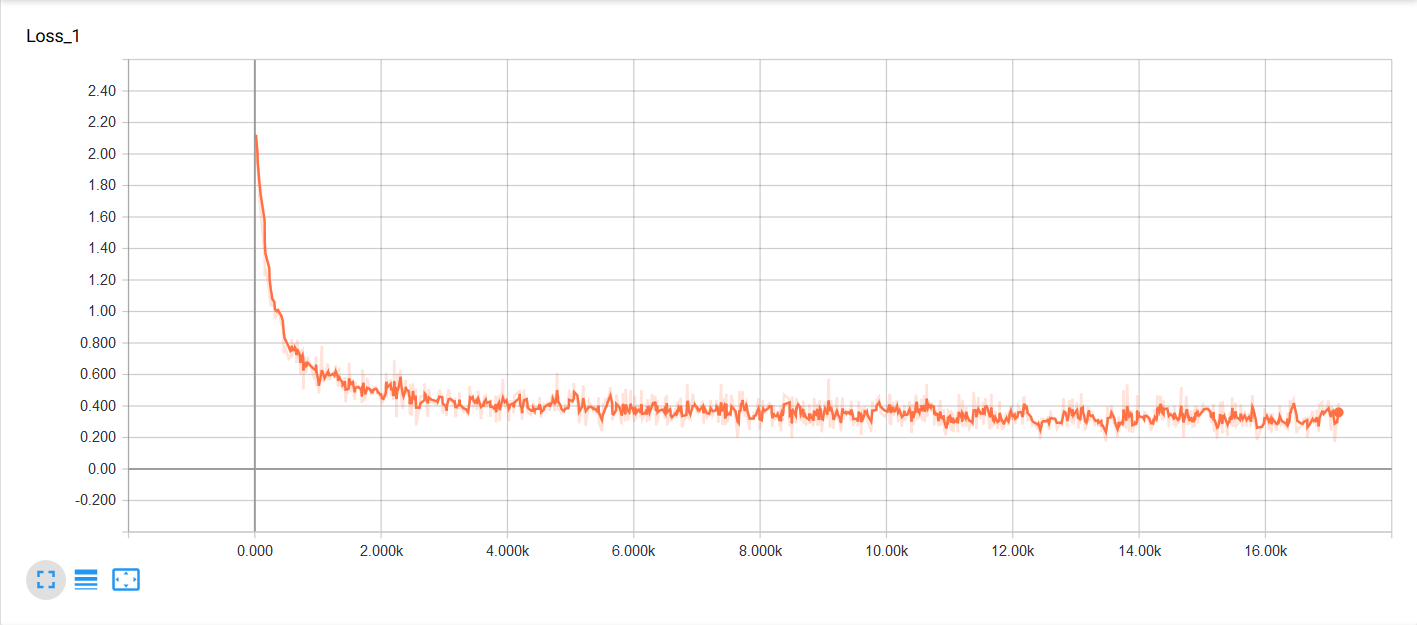
\includegraphics{./MNIST_figures/LossMLP.png}
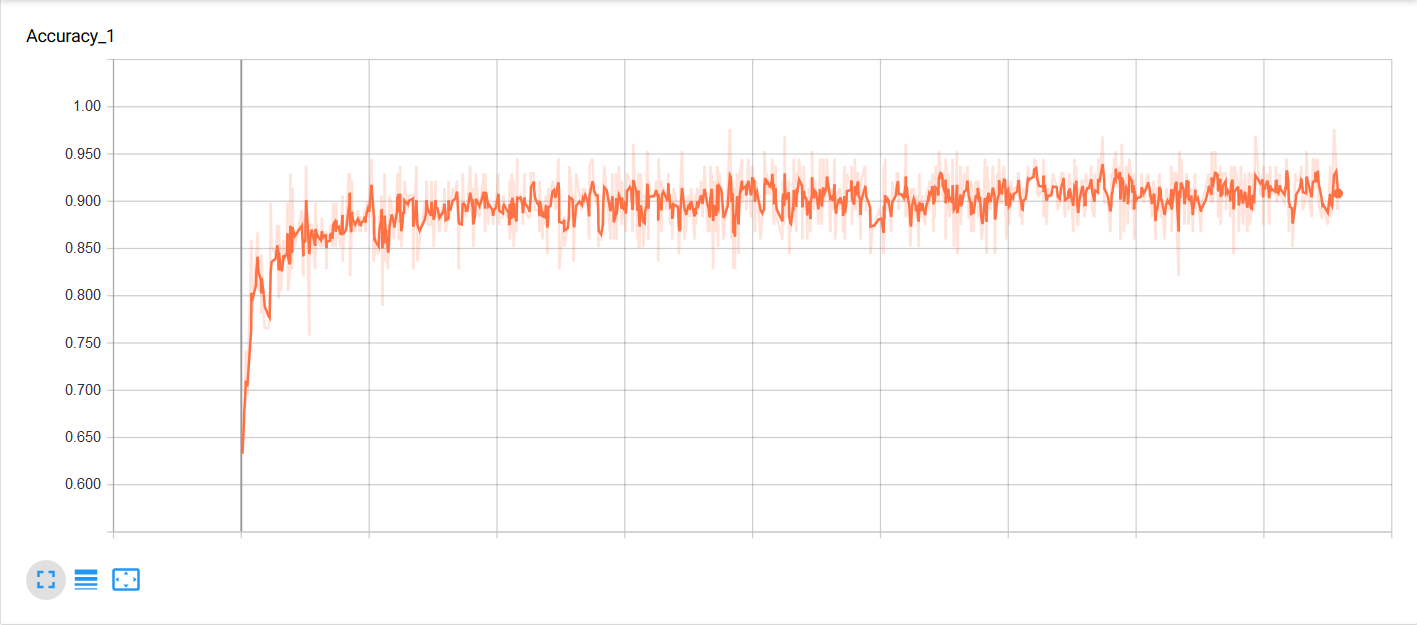
\includegraphics{./MNIST_figures/AccuracyMLP.png}
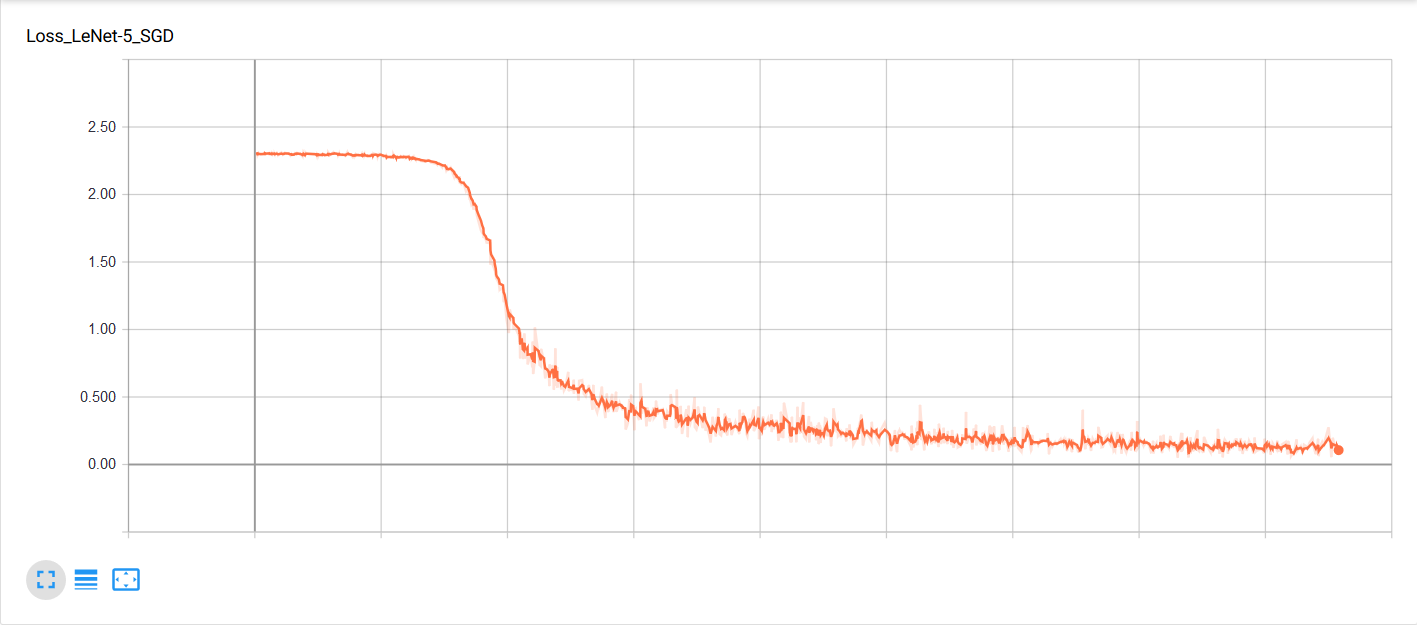
\includegraphics{./MNIST_figures/LossSGD.png}
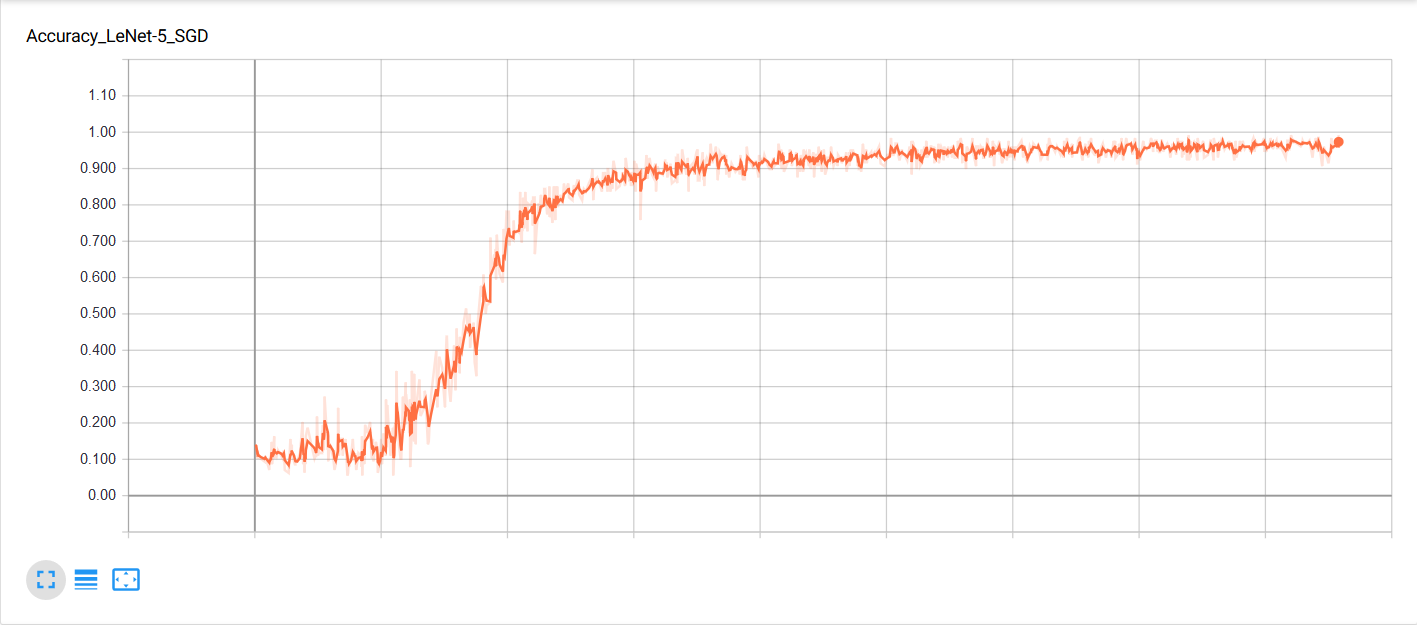
\includegraphics{./MNIST_figures/AccuracySGD.png}

We divided the error by more than two, this is a huge improvment. The
number of iterations seems good, as both accuracy and loss curves are
flattening at the end of the training. We can notice that for LeNet
optimization, the loss function is slow to decrease, but become very low
when it starts to do so.

     Part 2 : LeNET 5 Optimization

     Question 2.2.1

\begin{itemize}
\tightlist
\item
  Retrain your network with AdamOptimizer and then fill the table above:
\end{itemize}

\begin{longtable}[c]{@{}lll@{}}
\toprule
Optimizer & Gradient Descent & AdamOptimizer\tabularnewline
\midrule
\endhead
Testing Accuracy & 0.966 & 0.983\tabularnewline
Training Time & 10min 01s & 10min 03s\tabularnewline
\bottomrule
\end{longtable}

\begin{itemize}
\tightlist
\item
  Which optimizer gives the best accuracy on test data?
\end{itemize}

Even if computation times are the same, not only Adam Optimizer (which
is an improvement of Adagrad) converges faster, but it also gives better
results when dealing with mnist with LeNet5 (it divides the number of
mistakes by exactly 2). The parameters such as the learning-rate aren't
tuned, but they are set by default to their initial paper optimum by
tensorflow. This time, the loss function decrease really fast and do not
wait a lot of iterations to do so.

For instance, Adam is set to:

\begin{Shaded}
\begin{Highlighting}[]
    \NormalTok{learning_rate}\OperatorTok{=}\FloatTok{0.001}\NormalTok{,}
    \NormalTok{beta1}\OperatorTok{=}\FloatTok{0.9}\NormalTok{,}
    \NormalTok{beta2}\OperatorTok{=}\FloatTok{0.999}\NormalTok{,}
    \NormalTok{epsilon}\OperatorTok{=}\FloatTok{1e-08}\NormalTok{,}
    \NormalTok{use_locking}\OperatorTok{=}\VariableTok{False}\NormalTok{,}
    \NormalTok{name}\OperatorTok{=}\StringTok{'Adam'}
\end{Highlighting}
\end{Shaded}

    \begin{Verbatim}[commandchars=\\\{\}]
{\color{incolor}In [{\color{incolor}11}]:} \PY{n}{tf}\PY{o}{.}\PY{n}{reset\PYZus{}default\PYZus{}graph}\PY{p}{(}\PY{p}{)}
         
         \PY{c+c1}{\PYZsh{} Model}
         \PY{n}{x} \PY{o}{=} \PY{n}{tf}\PY{o}{.}\PY{n}{placeholder}\PY{p}{(}\PY{n}{tf}\PY{o}{.}\PY{n}{float32}\PY{p}{,} \PY{n}{shape}\PY{o}{=}\PY{p}{(}\PY{k+kc}{None}\PY{p}{,} \PY{l+m+mi}{784}\PY{p}{)}\PY{p}{,} \PY{n}{name}\PY{o}{=}\PY{l+s+s1}{\PYZsq{}}\PY{l+s+s1}{InputData}\PY{l+s+s1}{\PYZsq{}}\PY{p}{)}
         \PY{n}{y} \PY{o}{=} \PY{n}{tf}\PY{o}{.}\PY{n}{placeholder}\PY{p}{(}\PY{n}{tf}\PY{o}{.}\PY{n}{float32}\PY{p}{,} \PY{n}{shape}\PY{o}{=}\PY{p}{(}\PY{k+kc}{None}\PY{p}{,} \PY{l+m+mi}{10}\PY{p}{)}\PY{p}{,} \PY{n}{name}\PY{o}{=}\PY{l+s+s1}{\PYZsq{}}\PY{l+s+s1}{LabelData}\PY{l+s+s1}{\PYZsq{}}\PY{p}{)}
         
         \PY{n}{modelADAM} \PY{o}{=} \PY{n}{LeNet5\PYZus{}Model}\PY{p}{(}\PY{n}{x}\PY{p}{)}
         
         \PY{k}{with} \PY{n}{tf}\PY{o}{.}\PY{n}{name\PYZus{}scope}\PY{p}{(}\PY{l+s+s1}{\PYZsq{}}\PY{l+s+s1}{Accuracy\PYZus{}ADAM}\PY{l+s+s1}{\PYZsq{}}\PY{p}{)}\PY{p}{:}
             \PY{n}{accuracyADAM} \PY{o}{=} \PY{n}{evaluate}\PY{p}{(}\PY{n}{modelADAM}\PY{p}{,} \PY{n}{y}\PY{p}{)}
         \PY{k}{with} \PY{n}{tf}\PY{o}{.}\PY{n}{name\PYZus{}scope}\PY{p}{(}\PY{l+s+s1}{\PYZsq{}}\PY{l+s+s1}{Loss\PYZus{}ADAM}\PY{l+s+s1}{\PYZsq{}}\PY{p}{)}\PY{p}{:}
             \PY{n}{costADAM} \PY{o}{=} \PY{n}{tf}\PY{o}{.}\PY{n}{reduce\PYZus{}mean}\PY{p}{(}\PY{o}{\PYZhy{}}\PY{n}{tf}\PY{o}{.}\PY{n}{reduce\PYZus{}sum}\PY{p}{(}\PY{n}{y}\PY{o}{*}\PY{n}{tf}\PY{o}{.}\PY{n}{log}\PY{p}{(}\PY{n}{tf}\PY{o}{.}\PY{n}{clip\PYZus{}by\PYZus{}value}\PY{p}{(}\PY{n}{modelADAM}\PY{p}{,} \PY{n}{epsilon}\PY{p}{,} \PY{l+m+mf}{1.0}\PY{p}{)}\PY{p}{)}\PY{p}{,} \PY{n}{reduction\PYZus{}indices}\PY{o}{=}\PY{l+m+mi}{1}\PY{p}{)}\PY{p}{)}
         \PY{k}{with} \PY{n}{tf}\PY{o}{.}\PY{n}{name\PYZus{}scope}\PY{p}{(}\PY{l+s+s1}{\PYZsq{}}\PY{l+s+s1}{Optimisation\PYZus{}ADAM}\PY{l+s+s1}{\PYZsq{}}\PY{p}{)}\PY{p}{:}
             \PY{n}{optimizerADAM} \PY{o}{=} \PY{n}{tf}\PY{o}{.}\PY{n}{train}\PY{o}{.}\PY{n}{AdamOptimizer}\PY{p}{(}\PY{n}{learning\PYZus{}rate}\PY{p}{)}\PY{o}{.}\PY{n}{minimize}\PY{p}{(}\PY{n}{costADAM}\PY{p}{)}
             
         \PY{c+c1}{\PYZsh{} Initializing the variables}
         \PY{n}{init} \PY{o}{=} \PY{n}{tf}\PY{o}{.}\PY{n}{global\PYZus{}variables\PYZus{}initializer}\PY{p}{(}\PY{p}{)}
         \PY{c+c1}{\PYZsh{} Create a summary to monitor cost tensor}
         \PY{n}{tf}\PY{o}{.}\PY{n}{summary}\PY{o}{.}\PY{n}{scalar}\PY{p}{(}\PY{l+s+s2}{\PYZdq{}}\PY{l+s+s2}{Loss\PYZus{}LeNet\PYZhy{}5\PYZus{}Adam}\PY{l+s+s2}{\PYZdq{}}\PY{p}{,} \PY{n}{costADAM}\PY{p}{)}
         \PY{c+c1}{\PYZsh{} Create a summary to monitor accuracy tensor}
         \PY{n}{tf}\PY{o}{.}\PY{n}{summary}\PY{o}{.}\PY{n}{scalar}\PY{p}{(}\PY{l+s+s2}{\PYZdq{}}\PY{l+s+s2}{Accuracy\PYZus{}LeNet\PYZhy{}5\PYZus{}Adam}\PY{l+s+s2}{\PYZdq{}}\PY{p}{,} \PY{n}{accuracyADAM}\PY{p}{)}
         \PY{c+c1}{\PYZsh{} Merge all summaries into a single op}
         \PY{n}{merged\PYZus{}summary\PYZus{}op} \PY{o}{=} \PY{n}{tf}\PY{o}{.}\PY{n}{summary}\PY{o}{.}\PY{n}{merge\PYZus{}all}\PY{p}{(}\PY{p}{)}
\end{Verbatim}


    \begin{Verbatim}[commandchars=\\\{\}]
{\color{incolor}In [{\color{incolor}12}]:} \PY{o}{\PYZpc{}\PYZpc{}}\PY{k}{time}
         with tf.Session() as sess:
             train(init, sess, logs\PYZus{}path, training\PYZus{}epochs, batch\PYZus{}size, optimizerADAM, costADAM, accuracyADAM, merged\PYZus{}summary\PYZus{}op) 
         print(\PYZdq{}Elapsed time:\PYZdq{})
\end{Verbatim}


    \begin{Verbatim}[commandchars=\\\{\}]
Epoch 10	- Training data loss = 0.000235501
		- Test data accuracy = 0.982
Epoch 20	- Training data loss = 0.000209198
		- Test data accuracy = 0.986
Epoch 30	- Training data loss = 0.000043319
		- Test data accuracy = 0.985
Epoch 40	- Training data loss = 0.000290127
		- Test data accuracy = 0.983
Final Accuracy=0.983
Elapsed time:
CPU times: user 56min 20s, sys: 14min 46s, total: 1h 11min 7s
Wall time: 10min 3s

    \end{Verbatim}

    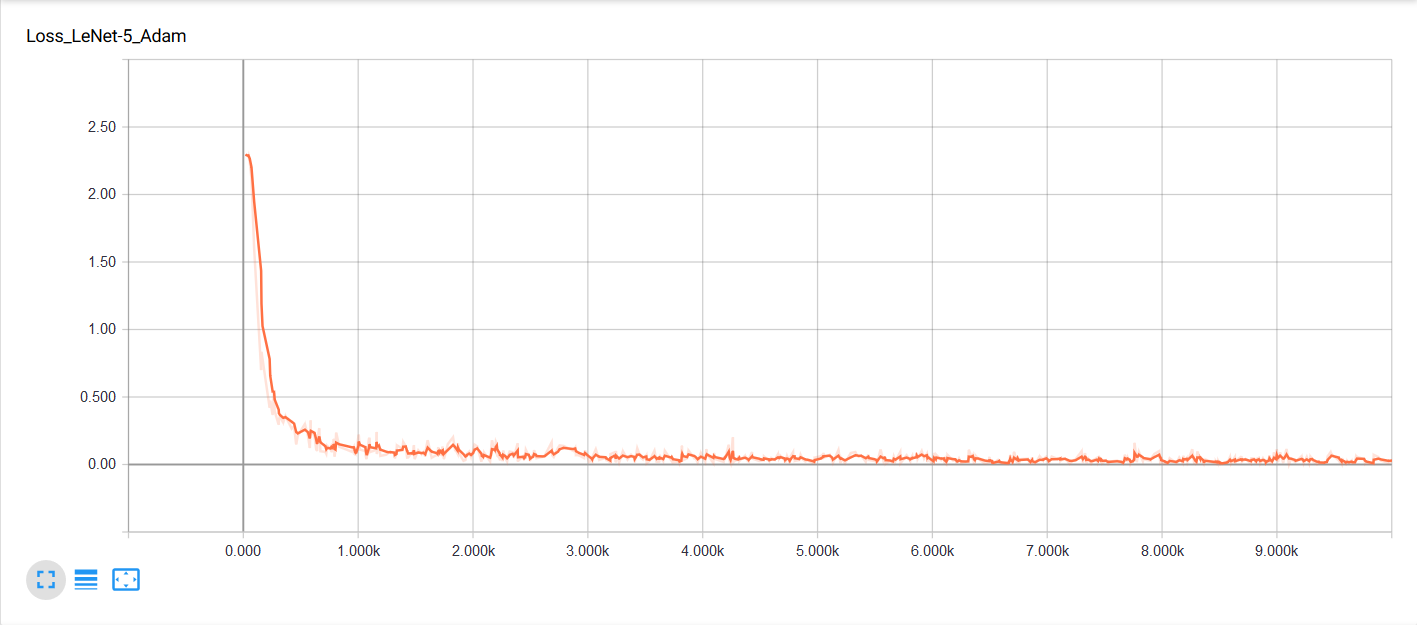
\includegraphics{./MNIST_figures/LossADAM.png}
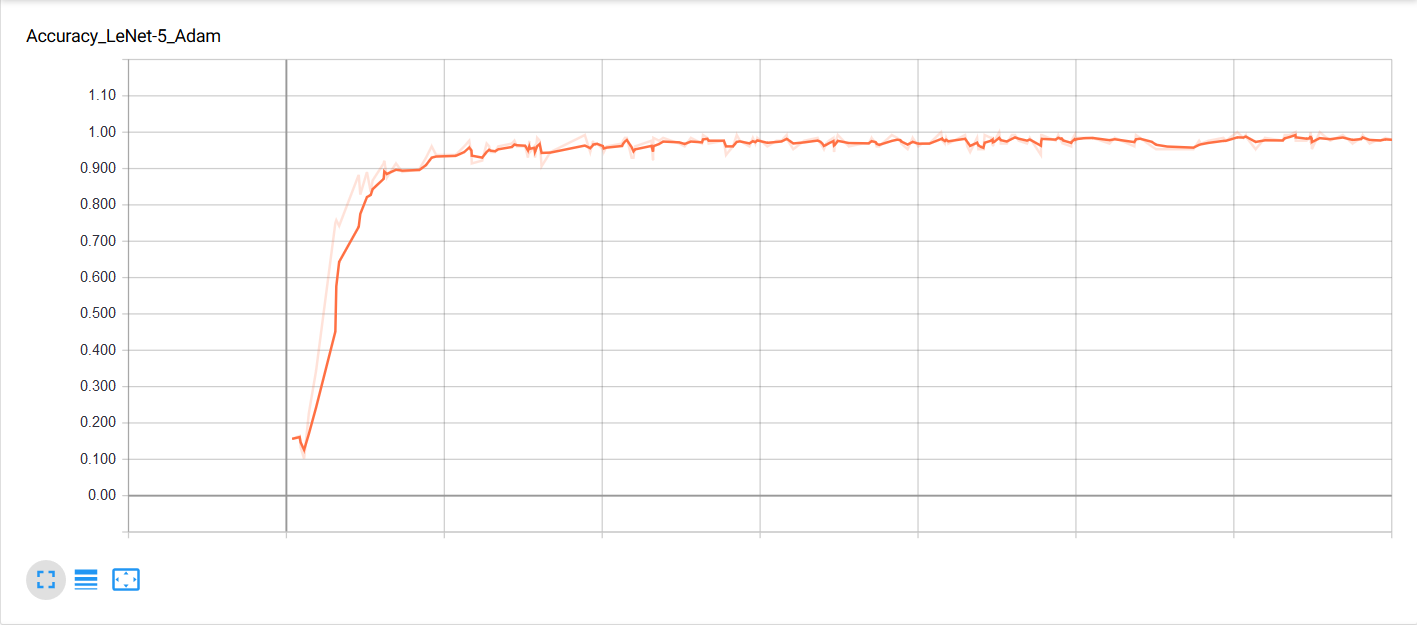
\includegraphics{./MNIST_figures/AccuracyADAM.png}

     Question 2.2.2 Try to add dropout (keep\_prob = 0.75) before the first
fully connected layer. You will use tf.nn.dropout for that purpose. What
accuracy do you achieve on testing data?

\textbf{Accuracy achieved on testing data:} 0.986 We have reduced our
number of errors by 15\%, which is significant. We are this time raising
the accuracy much faster.

    \begin{Verbatim}[commandchars=\\\{\}]
{\color{incolor}In [{\color{incolor}13}]:} \PY{k}{def} \PY{n+nf}{LeNet5\PYZus{}Model\PYZus{}Dropout}\PY{p}{(}\PY{o}{*}\PY{n}{args}\PY{p}{,} \PY{o}{*}\PY{o}{*}\PY{n}{kwargs}\PY{p}{)}\PY{p}{:}    
             \PY{k}{return} \PY{n}{LeNet5\PYZus{}Model}\PY{p}{(}\PY{o}{*}\PY{n}{args}\PY{p}{,} \PY{o}{*}\PY{o}{*}\PY{n}{kwargs}\PY{p}{,} \PY{n}{dropout}\PY{o}{=}\PY{k+kc}{True}\PY{p}{)}
\end{Verbatim}


    \begin{Verbatim}[commandchars=\\\{\}]
{\color{incolor}In [{\color{incolor}14}]:} \PY{n}{tf}\PY{o}{.}\PY{n}{reset\PYZus{}default\PYZus{}graph}\PY{p}{(}\PY{p}{)}
         
         \PY{c+c1}{\PYZsh{} Model}
         \PY{n}{x} \PY{o}{=} \PY{n}{tf}\PY{o}{.}\PY{n}{placeholder}\PY{p}{(}\PY{n}{tf}\PY{o}{.}\PY{n}{float32}\PY{p}{,} \PY{n}{shape}\PY{o}{=}\PY{p}{(}\PY{k+kc}{None}\PY{p}{,} \PY{l+m+mi}{784}\PY{p}{)}\PY{p}{,} \PY{n}{name}\PY{o}{=}\PY{l+s+s1}{\PYZsq{}}\PY{l+s+s1}{InputData}\PY{l+s+s1}{\PYZsq{}}\PY{p}{)}
         \PY{n}{y} \PY{o}{=} \PY{n}{tf}\PY{o}{.}\PY{n}{placeholder}\PY{p}{(}\PY{n}{tf}\PY{o}{.}\PY{n}{float32}\PY{p}{,} \PY{n}{shape}\PY{o}{=}\PY{p}{(}\PY{k+kc}{None}\PY{p}{,} \PY{l+m+mi}{10}\PY{p}{)}\PY{p}{,} \PY{n}{name}\PY{o}{=}\PY{l+s+s1}{\PYZsq{}}\PY{l+s+s1}{LabelData}\PY{l+s+s1}{\PYZsq{}}\PY{p}{)}
         
         \PY{n}{modelDrop} \PY{o}{=} \PY{n}{LeNet5\PYZus{}Model\PYZus{}Dropout}\PY{p}{(}\PY{n}{x}\PY{p}{)}
         
         \PY{k}{with} \PY{n}{tf}\PY{o}{.}\PY{n}{name\PYZus{}scope}\PY{p}{(}\PY{l+s+s1}{\PYZsq{}}\PY{l+s+s1}{Accuracy\PYZus{}DROPOUT}\PY{l+s+s1}{\PYZsq{}}\PY{p}{)}\PY{p}{:}
             \PY{n}{accuracyDROP} \PY{o}{=} \PY{n}{evaluate}\PY{p}{(}\PY{n}{modelDrop}\PY{p}{,} \PY{n}{y}\PY{p}{)}
         \PY{k}{with} \PY{n}{tf}\PY{o}{.}\PY{n}{name\PYZus{}scope}\PY{p}{(}\PY{l+s+s1}{\PYZsq{}}\PY{l+s+s1}{Loss\PYZus{}DROPOUT}\PY{l+s+s1}{\PYZsq{}}\PY{p}{)}\PY{p}{:}
             \PY{n}{costDROP} \PY{o}{=} \PY{n}{tf}\PY{o}{.}\PY{n}{reduce\PYZus{}mean}\PY{p}{(}\PY{o}{\PYZhy{}}\PY{n}{tf}\PY{o}{.}\PY{n}{reduce\PYZus{}sum}\PY{p}{(}\PY{n}{y}\PY{o}{*}\PY{n}{tf}\PY{o}{.}\PY{n}{log}\PY{p}{(}\PY{n}{tf}\PY{o}{.}\PY{n}{clip\PYZus{}by\PYZus{}value}\PY{p}{(}\PY{n}{modelDrop}\PY{p}{,} \PY{n}{epsilon}\PY{p}{,} \PY{l+m+mf}{1.0}\PY{p}{)}\PY{p}{)}\PY{p}{,} \PY{n}{reduction\PYZus{}indices}\PY{o}{=}\PY{l+m+mi}{1}\PY{p}{)}\PY{p}{)}
         \PY{k}{with} \PY{n}{tf}\PY{o}{.}\PY{n}{name\PYZus{}scope}\PY{p}{(}\PY{l+s+s1}{\PYZsq{}}\PY{l+s+s1}{Optimisation\PYZus{}DROPOUT}\PY{l+s+s1}{\PYZsq{}}\PY{p}{)}\PY{p}{:}
             \PY{n}{optimizerDROP} \PY{o}{=} \PY{n}{tf}\PY{o}{.}\PY{n}{train}\PY{o}{.}\PY{n}{AdamOptimizer}\PY{p}{(}\PY{n}{learning\PYZus{}rate}\PY{p}{)}\PY{o}{.}\PY{n}{minimize}\PY{p}{(}\PY{n}{costDROP}\PY{p}{)}
             
         \PY{c+c1}{\PYZsh{} Initializing the variables}
         \PY{n}{init} \PY{o}{=} \PY{n}{tf}\PY{o}{.}\PY{n}{global\PYZus{}variables\PYZus{}initializer}\PY{p}{(}\PY{p}{)}
         \PY{c+c1}{\PYZsh{} Create a summary to monitor cost tensor}
         \PY{n}{tf}\PY{o}{.}\PY{n}{summary}\PY{o}{.}\PY{n}{scalar}\PY{p}{(}\PY{l+s+s2}{\PYZdq{}}\PY{l+s+s2}{Loss\PYZus{}LeNet\PYZhy{}5\PYZus{}Drop}\PY{l+s+s2}{\PYZdq{}}\PY{p}{,} \PY{n}{costDROP}\PY{p}{)}
         \PY{c+c1}{\PYZsh{} Create a summary to monitor accuracy tensor}
         \PY{n}{tf}\PY{o}{.}\PY{n}{summary}\PY{o}{.}\PY{n}{scalar}\PY{p}{(}\PY{l+s+s2}{\PYZdq{}}\PY{l+s+s2}{Accuracy\PYZus{}LeNet\PYZhy{}5\PYZus{}Drop}\PY{l+s+s2}{\PYZdq{}}\PY{p}{,} \PY{n}{accuracyDROP}\PY{p}{)}
         \PY{c+c1}{\PYZsh{} Merge all summaries into a single op}
         \PY{n}{merged\PYZus{}summary\PYZus{}op} \PY{o}{=} \PY{n}{tf}\PY{o}{.}\PY{n}{summary}\PY{o}{.}\PY{n}{merge\PYZus{}all}\PY{p}{(}\PY{p}{)}
\end{Verbatim}


    \begin{Verbatim}[commandchars=\\\{\}]
{\color{incolor}In [{\color{incolor}15}]:} \PY{o}{\PYZpc{}\PYZpc{}}\PY{k}{time}
         with tf.Session() as sess:
             train(init, sess, logs\PYZus{}path, training\PYZus{}epochs, batch\PYZus{}size, optimizerDROP, costDROP, accuracyDROP, merged\PYZus{}summary\PYZus{}op) 
         print(\PYZdq{}Elapsed time:\PYZdq{})
\end{Verbatim}


    \begin{Verbatim}[commandchars=\\\{\}]
Epoch 10	- Training data loss = 0.000125411
		- Test data accuracy = 0.978
Epoch 20	- Training data loss = 0.000041697
		- Test data accuracy = 0.982
Epoch 30	- Training data loss = 0.000018722
		- Test data accuracy = 0.985
Epoch 40	- Training data loss = 0.000032723
		- Test data accuracy = 0.984
Final Accuracy=0.986
Elapsed time:
CPU times: user 57min 4s, sys: 12min 9s, total: 1h 9min 14s
Wall time: 10min 14s

    \end{Verbatim}

    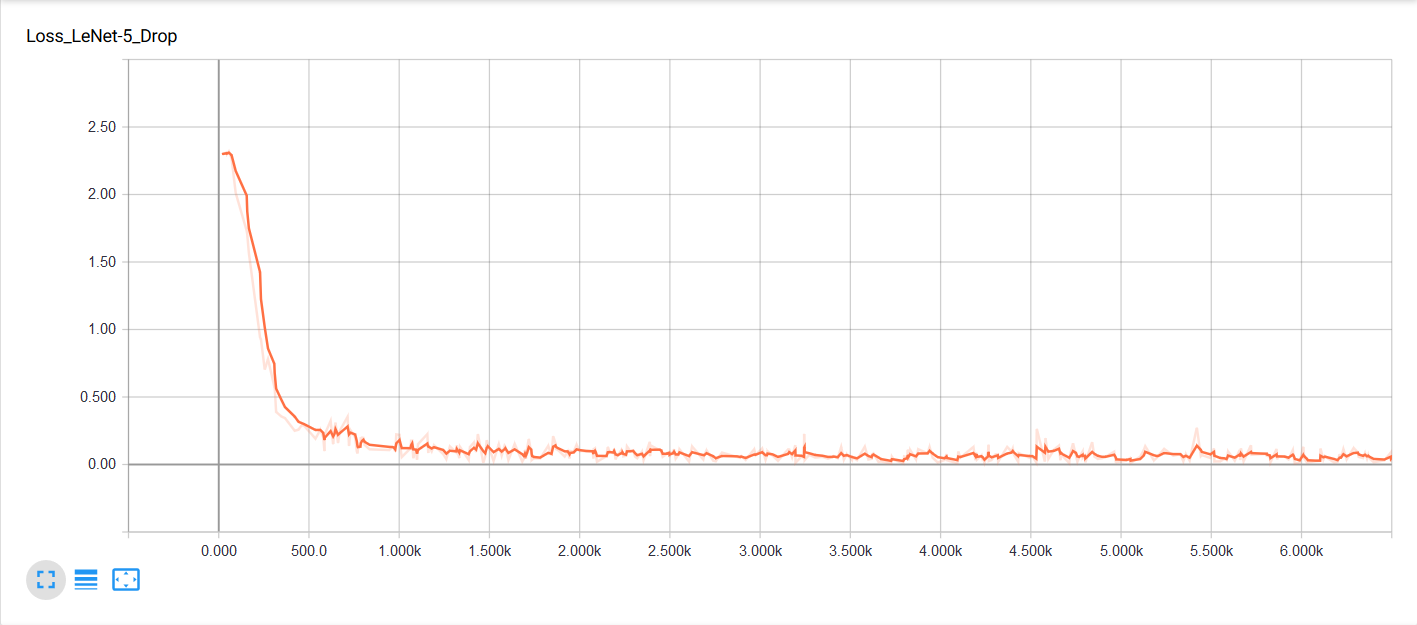
\includegraphics{./MNIST_figures/LossDROP.png}
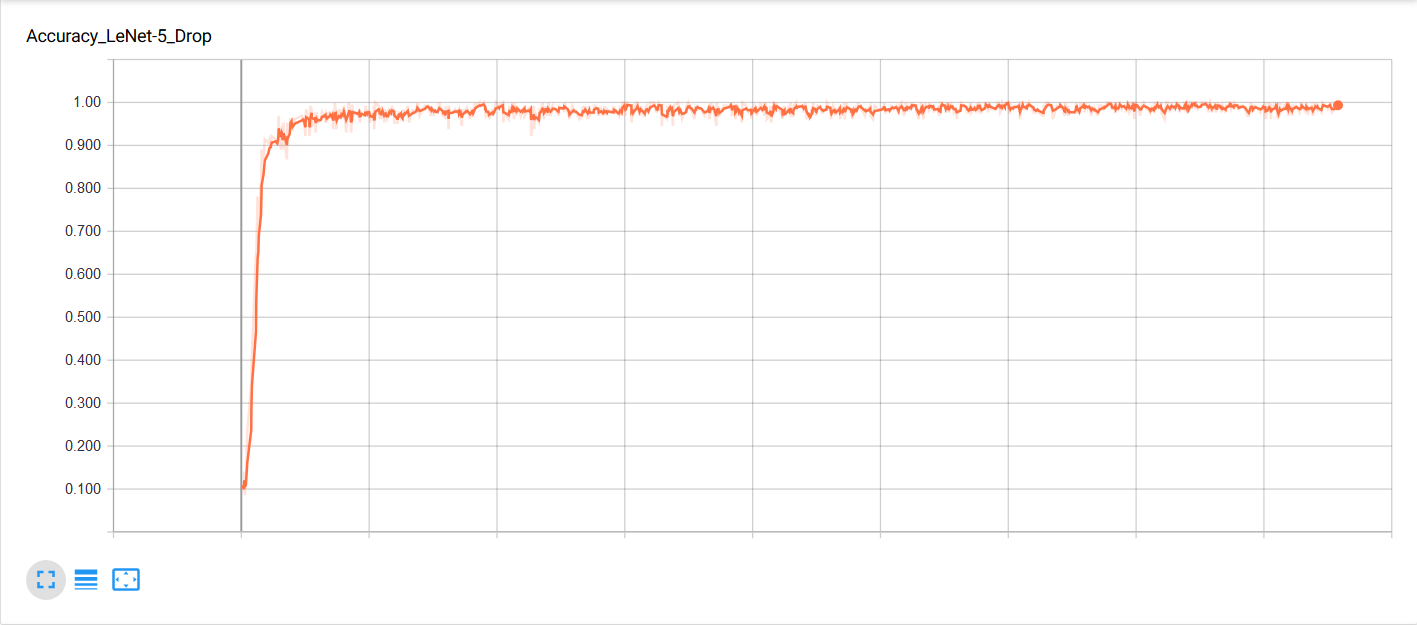
\includegraphics{./MNIST_figures/AccuracyDROP.png}


    % Add a bibliography block to the postdoc
    
    
    
    \end{document}
